\chapter{実験}
\label{chap:poordirection}

\section{実験結果}

\subsection{数値データによる結果}
数値データを用いた精度(正解率・適合率・再現率・F値)を表\ref{value_hatoma}、表\ref{value_kurosima}に示す。また、西表大原航路、小浜航路、竹富航路では欠航データが無く精度が100\%となったので省く、波照間航路や西表上原航路は表\ref{value_hatoma}のような傾向と似ている結果となったため省く。


\begin{table}[htbp]
  \begin{center}
    \begin{tabular}{c}
	%1
      \begin{minipage}{0.5\hsize}
        \begin{center}
          \caption{鳩間島航路-鳩間発}
          \begin{tabular}{|c|r|r|r|r|} \hline
   &正解率 & 適合率 & 再現率 & F値 \\ \hline
      当日&0.868 &0.933 &0.778 &0.848 \\ \hline
     1日前 & 0.816 & 0.875 & 0.737 & 0.800 \\ \hline
      2日前 & 0.816 & 0.929 & 0.684 & 0.788 \\ \hline
      3日前 & 0.649 & 0.636 & 0.737 & 0.683 \\ \hline 
      4日前 & 0.757 & 0.737 & 0.778 & 0.757 \\ \hline 
      5日前 & 0.639 & 0.667 & 0.556 & 0.667 \\ \hline 
      6日前 & 0.722 & 0.833 & 0.556 & 0.667 \\ \hline 
      7日前 & 0.583 & 0.562 & 0.529 & 0.545 \\ \hline 
      8日前 & 0.714 & 0.733 & 0.647 & 0.688 \\ \hline 
      9日前 & 0.629 & 0.625 & 0.588 & 0.606 \\ \hline 
          \end{tabular}
          \label{value_hatoma}
        \end{center}
      \end{minipage}
      %2
      \begin{minipage}{0.5\hsize}
        \begin{center}
          \caption{黒島航路-黒島発}
    \begin{tabular}{|c|r|r|r|r|} \hline
   &正解率 & 適合率 & 再現率 & F値 \\ \hline
      当日 & 1.000 & 1.000 & 1.000 & 1.000 \\ \hline
     1日前 & 0.987 & 0.000& 0.000 & 0.000 \\ \hline
      2日前 & 1.000 & 1.000 & 1.000 & 1.000 \\ \hline
      3日前 & 0.986 & 0.000 & 0.000 & 0.000 \\ \hline 
      4日前 & 1.000 & 0.000 & 0.000 & 0.000 \\ \hline 
      5日前 & 0.986 & 0.000 & 0.000 & 0.000 \\ \hline 
      6日前 & 0.986 & 0.000 & 0.000 & 0.000 \\ \hline 
      7日前 & 0.986 & 0.000 & 0.000 & 0.000 \\ \hline 
      8日前 & 1.000 & 1.000 & 1.000 & 1.000 \\ \hline 
      9日前 & 0.986 & 0.000 & 0.000 & 0.000 \\ \hline 
          \end{tabular}
           \label{value_kurosima}
        \end{center}
      \end{minipage}

    \end{tabular}
  \end{center}
\end{table}




\subsection{画像データによる結果}
画像データの波高レイヤーデータを用いた精度(正解率・適合率・再現率・F値)を表\ref{img_wave_hateruma}、表\ref{img_wave_hatoma}、表\ref{img_wave_taketomi}に示す。また、小浜島航路、黒島航路、西表大原航路は表\ref{img_wave_taketomi}と同様の結果が出力されたため省く、西表上原航路は表\ref{img_wave_hatoma}と傾向が似ているため省く。


\begin{table}[htbp]
  \begin{center}
    \begin{tabular}{c}
	%1
      \begin{minipage}{0.5\hsize}
        \begin{center}
          \caption{波高レイヤー(波照間航路-波照発)}
          \begin{tabular}{|c|r|r|r|r|} \hline
   &正解率 & 適合率 & 再現率 & F値 \\ \hline
      当日&0.796 &0.643 &0.643 &0.643 \\ \hline
     1日前 & 0.833 & 0.857 & 0.462 & 0.600 \\ \hline
      2日前 & 0.723 & 0.000 & 0.000 & 0.000 \\ \hline
      3日前 & 0.723 & 0.000 & 0.000 & 0.000 \\ \hline 
      4日前 & 0.756 & 0.000 & 0.000 & 0.000 \\ \hline 
      5日前 & 0.778 & 0.000 & 0.000 & 0.000 \\ \hline 
      6日前 & 0.773 & 0.000 & 0.000 & 0.000 \\ \hline 
      7日前 & 0.773 & 0.000 & 0.000 & 0.000 \\ \hline 
      8日前 & 0.773 & 0.000 & 0.000 & 0.000 \\ \hline 
      9日前 & 0.767 & 0.000 & 0.000 & 0.000 \\ \hline 
          \end{tabular}
          \label{img_wave_hateruma}
        \end{center}
      \end{minipage}
      %2
      \begin{minipage}{0.5\hsize}
        \begin{center}
          \caption{波高レイヤー(鳩間島航路-鳩間発)}
    \begin{tabular}{|c|r|r|r|r|} \hline
   &正解率 & 適合率 & 再現率 & F値 \\ \hline
      当日 & 0.882 & 0.929 & 0.812 & 0.867 \\ \hline
     1日前 & 0.818 & 0.917 & 0.688 & 0.786 \\ \hline
      2日前 & 0.727 & 0.818 & 0.562 & 0.667 \\ \hline
      3日前 & 0.562 & 0.545 & 0.400 & 0.462 \\ \hline 
      4日前 & 0.594 & 0.538 & 0.500 & 0.519 \\ \hline 
      5日前 & 0.645 & 0.615 & 0.571 & 0.593 \\ \hline 
      6日前 & 0.613 & 0.600 & 0.429 & 0.500 \\ \hline 
      7日前 & 0.581 & 0.545 & 0.429 & 0.480 \\ \hline 
      8日前 & 0.700 & 0.647 & 0.786 & 0.710 \\ \hline 
      9日前 & 0.667 & 0.667 & 0.571 & 0.615 \\ \hline 
          \end{tabular}
          \label{img_wave_hatoma}
        \end{center}
      \end{minipage}

    \end{tabular}
  \end{center}
\end{table}

\begin{table}[H]
  \begin{center}
    \caption{波高レイヤー(竹富航路-竹富発)}
    \begin{tabular}{|c|r|r|r|r|} \hline
   &正解率 & 適合率 & 再現率 & F値 \\ \hline
      当日 & 0.990 & 0.000 & 0.000 & 0.000 \\ \hline
     1日前 & 0.979 & 0.000 & 0.000 & 0.000 \\ \hline
      2日前 & 0.974 & 0.000 & 0.000 & 0.000 \\ \hline
      3日前 & 0.973 & 0.000 & 0.000 & 0.000 \\ \hline 
      4日前 & 0.972 & 0.000 & 0.000 & 0.000 \\ \hline 
      5日前 & 0.972 & 0.000 & 0.000 & 0.000 \\ \hline 
      6日前 & 0.977 & 0.000 & 0.000 & 0.000 \\ \hline 
      7日前 & 0.989 & 0.000 & 0.000 & 0.000 \\ \hline 
      8日前 & 0.994 & 0.000 & 0.000 & 0.000 \\ \hline 
      9日前 & 0.994 & 0.000 & 0.000 & 0.000 \\ \hline 
    \end{tabular}    
    \label{img_wave_taketomi}
  \end{center}
\end{table}

画像データの風速レイヤーデータを用いた精度(正解率・適合率・再現率・F値)を表\ref{img_wind_hateruma}、表\ref{img_wind_iriue}、表\ref{img_wind_taketomi}に示す。また、小浜島航路、黒島航路、西表大原航路は表\ref{img_wind_iriue}と同様の結果が出力されたため省く、鳩間島航路は表\ref{img_wind_iriue}と傾向が似ているため省く。

\begin{table}[htbp]
  \begin{center}
    \begin{tabular}{c}
	%1
      \begin{minipage}{0.5\hsize}
        \begin{center}
          \caption{風速レイヤー(波照間航路-波照発)}
          \begin{tabular}{|c|r|r|r|r|} \hline
   &正解率 & 適合率 & 再現率 & F値 \\ \hline
      当日&0.776 &0.579 &0.786 &0.667 \\ \hline
     1日前 & 0.812 & 0.750 & 0.462 & 0.571 \\ \hline
      2日前 & 0.729 & 0.000 & 0.000 & 0.000 \\ \hline
      3日前 & 0.723 & 0.000 & 0.000 & 0.000 \\ \hline 
      4日前 & 0.756 & 0.000 & 0.000 & 0.000 \\ \hline 
      5日前 & 0.778 & 0.000 & 0.000 & 0.000 \\ \hline 
      6日前 & 0.773 & 0.000 & 0.000 & 0.000 \\ \hline 
      7日前 & 0.773 & 0.000 & 0.000 & 0.000 \\ \hline 
      8日前 & 0.750 & 0.000 & 0.000 & 0.000 \\ \hline 
      9日前 & 0.767 & 0.000 & 0.000 & 0.000 \\ \hline 
          \end{tabular}
          \label{img_wind_hateruma}
        \end{center}
      \end{minipage}
      %2
      \begin{minipage}{0.5\hsize}
        \begin{center}
          \caption{風速レイヤー(西表上原航路-西表上原発)}
    \begin{tabular}{|c|r|r|r|r|} \hline
   &正解率 & 適合率 & 再現率 & F値 \\ \hline
      当日 & 0.846 & 0.863 & 0.786 & 0.822 \\ \hline
     1日前 & 0.803 & 0.971 & 0.589 & 0.733 \\ \hline
      2日前 & 0.708 & 0.769 & 0.536 & 0.632 \\ \hline
      3日前 & 0.619 & 0.610 & 0.463 & 0.526 \\ \hline 
      4日前 & 0.696 & 0.684 & 0.531 & 0.598 \\ \hline 
      5日前 & 0.649 & 0.610 & 0.510 & 0.556 \\ \hline 
      6日前 & 0.598 & 0.562 & 0.367 & 0.444 \\ \hline 
      7日前 & 0.527 & 0.429 & 0.180 & 0.254 \\ \hline 
      8日前 & 0.709 & 0.630 & 0.902 & 0.742 \\ \hline 
      9日前 & 0.697 & 0.638 & 0.755 & 0.692 \\ \hline 
          \end{tabular}
          \label{img_wind_iriue}
        \end{center}
      \end{minipage}

    \end{tabular}
  \end{center}
\end{table}

\begin{table}[H]
  \begin{center}
    \caption{風速レイヤー(竹富航路-竹富発)}
    \begin{tabular}{|c|r|r|r|r|} \hline
   &正解率 & 適合率 & 再現率 & F値 \\ \hline
      当日 & 0.990 & 0.000 & 0.000 & 0.000 \\ \hline
     1日前 & 0.979 & 0.000 & 0.000 & 0.000 \\ \hline
      2日前 & 0.974 & 0.000 & 0.000 & 0.000 \\ \hline
      3日前 & 0.973 & 0.000 & 0.000 & 0.000 \\ \hline 
      4日前 & 0.978 & 0.000 & 0.000 & 0.000 \\ \hline 
      5日前 & 0.989 & 1.000 & 0.600 & 0.750 \\ \hline 
      6日前 & 0.978 & 0.000 & 0.000 & 0.000 \\ \hline 
      7日前 & 0.989 & 0.000 & 0.000 & 0.000 \\ \hline 
      8日前 & 0.994 & 0.000 & 0.000 & 0.000 \\ \hline 
      9日前 & 0.994 & 0.000 & 0.000 & 0.000 \\ \hline 
    \end{tabular}
    \label{img_wind_taketomi}
  \end{center}
\end{table}


\section{考察}

\subsection{数値データの考察}

表\ref{value_hatoma}の鳩間島航路-鳩間発1日前モデルにおけるテストデータの予測結果別に色分けをした散布図が図\ref{hatoma_1_scatter_pred}になる。この図を見ると特徴量wave\_heightの箇所で明確な色分けがおこなわれているのが確認でき、教師ラベルとの強い関係性を見ることができる。この結果から1日前モデルがwave\_heightを重要な特徴量として処理していると考えられる。
そこで、9日前モデルの散布図\ref{hatoma_9_scatter_pred}を見ると各特徴量と教師データとの結びつきが弱くなっていることが確認できる。そのため9日前モデルでは表\ref{value_hatoma}で示されているように予測精度が悪くなっていることが説明できる。これはデータセット作成する際、特徴量と教師ラベルを9日間ずらして作成しているため、1日前と比較して特徴量が運航や欠航を説明するための情報が減少していると考えられる。

\begin{figure}[H]
 \centering
 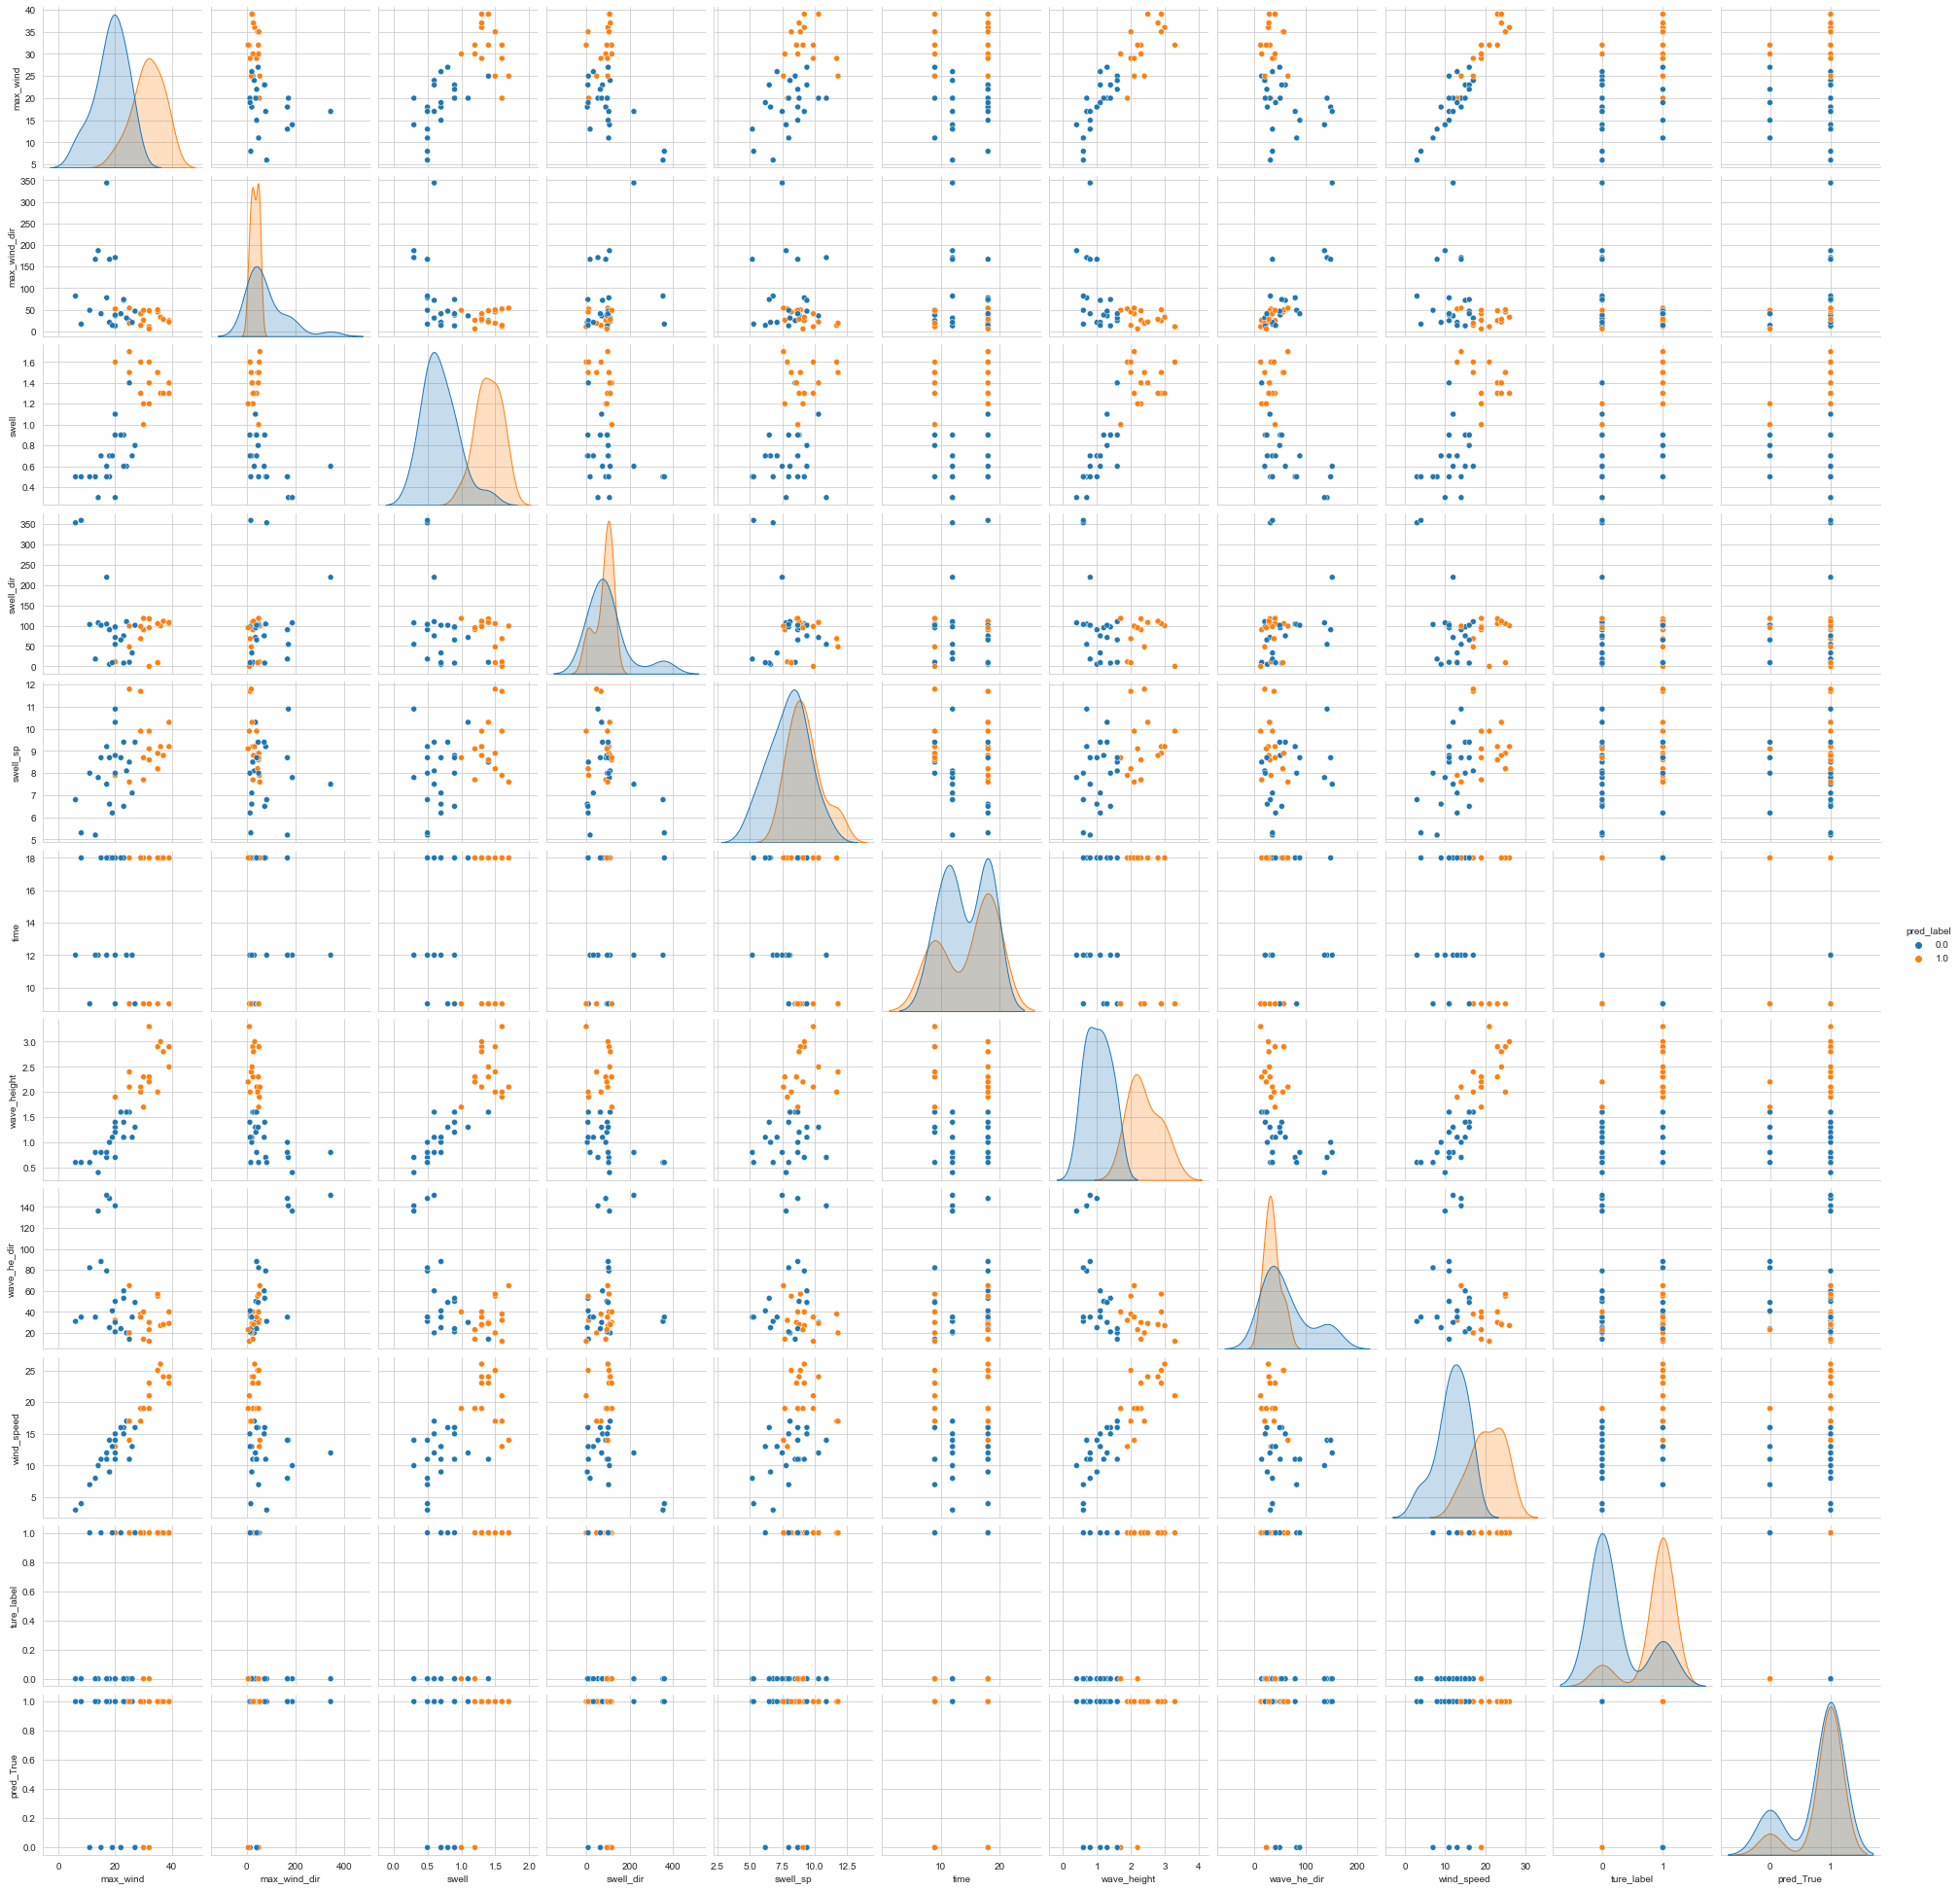
\includegraphics[keepaspectratio, scale=0.25]{fig/chapter4/hatoma_1_pred.png}
 \caption{鳩間島航路1日前モデルの予測ラベル}
 \label{hatoma_1_scatter_pred}
\end{figure}

\begin{figure}[H]
 \centering
 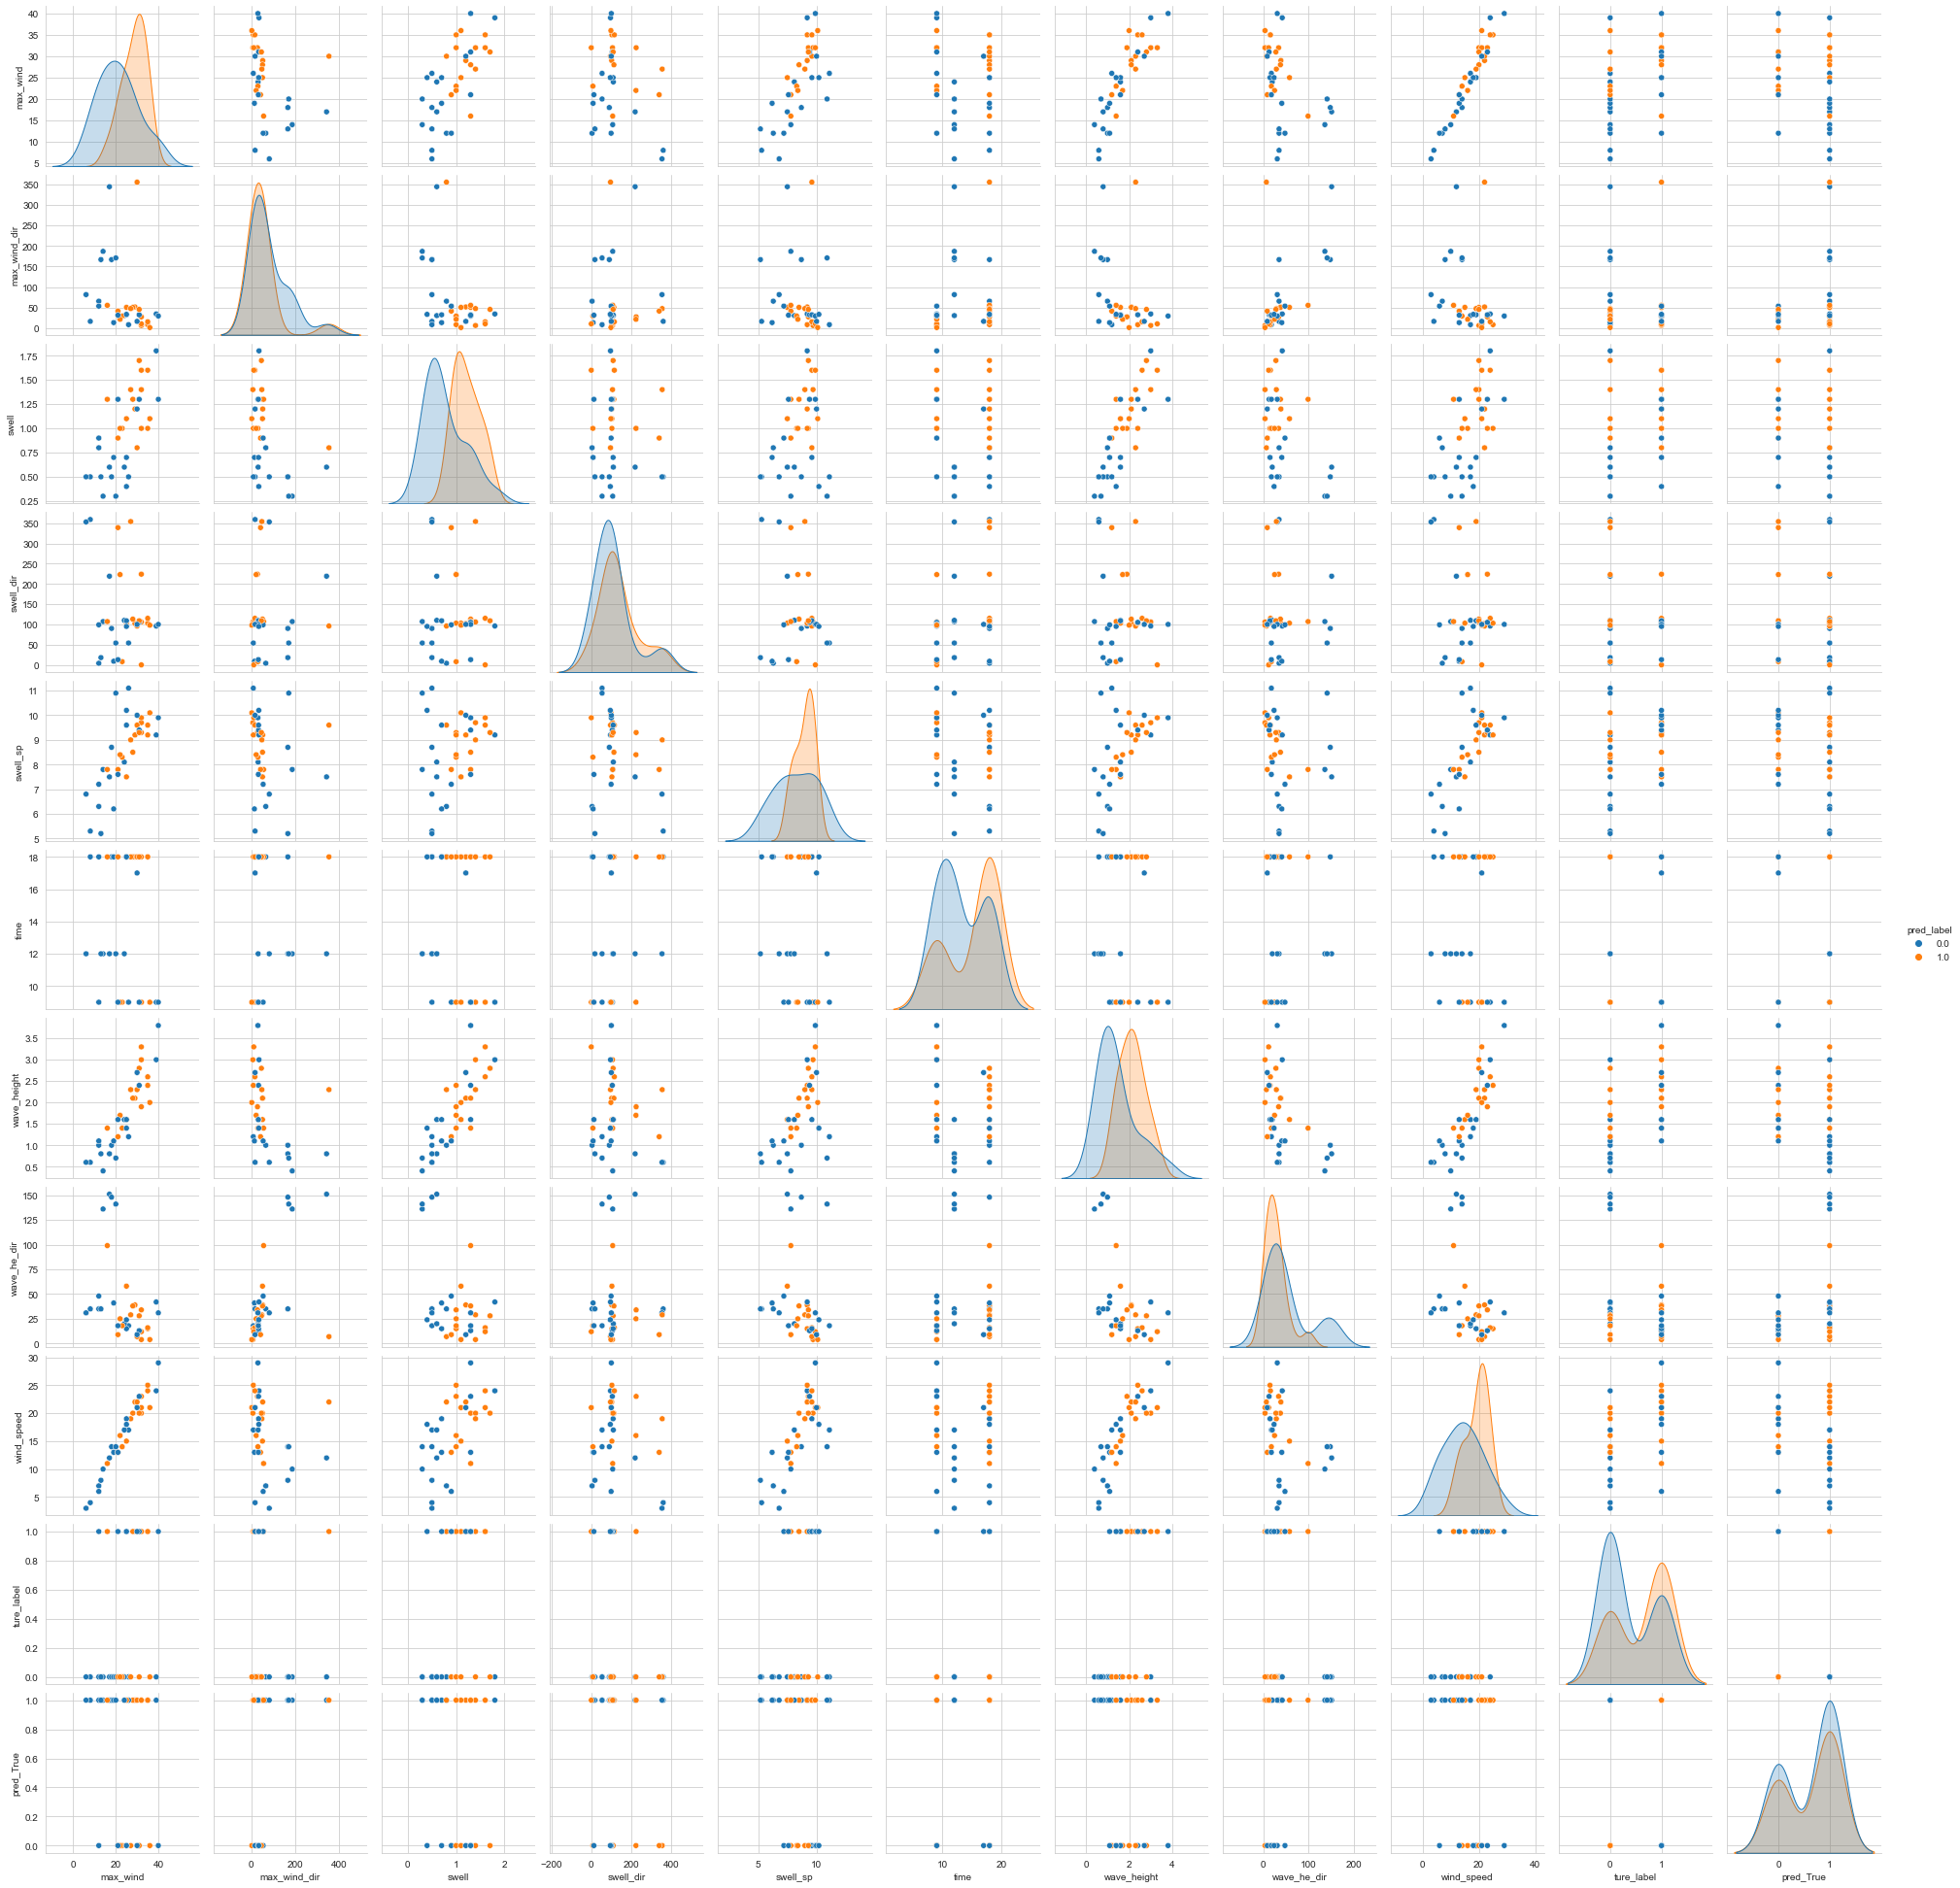
\includegraphics[keepaspectratio, scale=0.25]{fig/chapter4/hatoma_9_pred.png}
 \caption{鳩間島航路9日前モデルの予測ラベル}
 \label{hatoma_9_scatter_pred}
\end{figure}

表\ref{value_kurosima}から黒島航路-黒島発当日モデルの結果では全ての評価指標において1.000を獲得しており精度がとても良いことがわかる。当日モデルのテストデータの予測結果別に色分けをした散布図\ref{kurosima_0_scatter_pred}を確認すると、テストデータにある唯一の欠航データの特徴をしっかり捉えて予測できたことが確認できる。しかし、表\ref{value_kurosima}の1日前モデルの評価結果では正解率0.987とよく見えるがF値が0.000となっており欠航データに対する予測が全くできていないことが見て取れる。散布図\ref{kurosima_1_scatter_pred}を見てもわかるように全て運航すると予測されている。そこで、1日前モデルで用いたテストデータの教師ラベルを真値で色分けした散布図\ref{kurosima_1_scatter_ture}を見ると欠航データであるオレンジ点が青色の運航データの集団の中に分布していることが確認できる。このことからデータセットの教師データを1日ずらしたモデルの1日前モデルではデータセットをずらすことで欠航という情報を維持できず、運航のデータと変わらないデータになっていることが考えられる。


\begin{figure}[H]
 \centering
 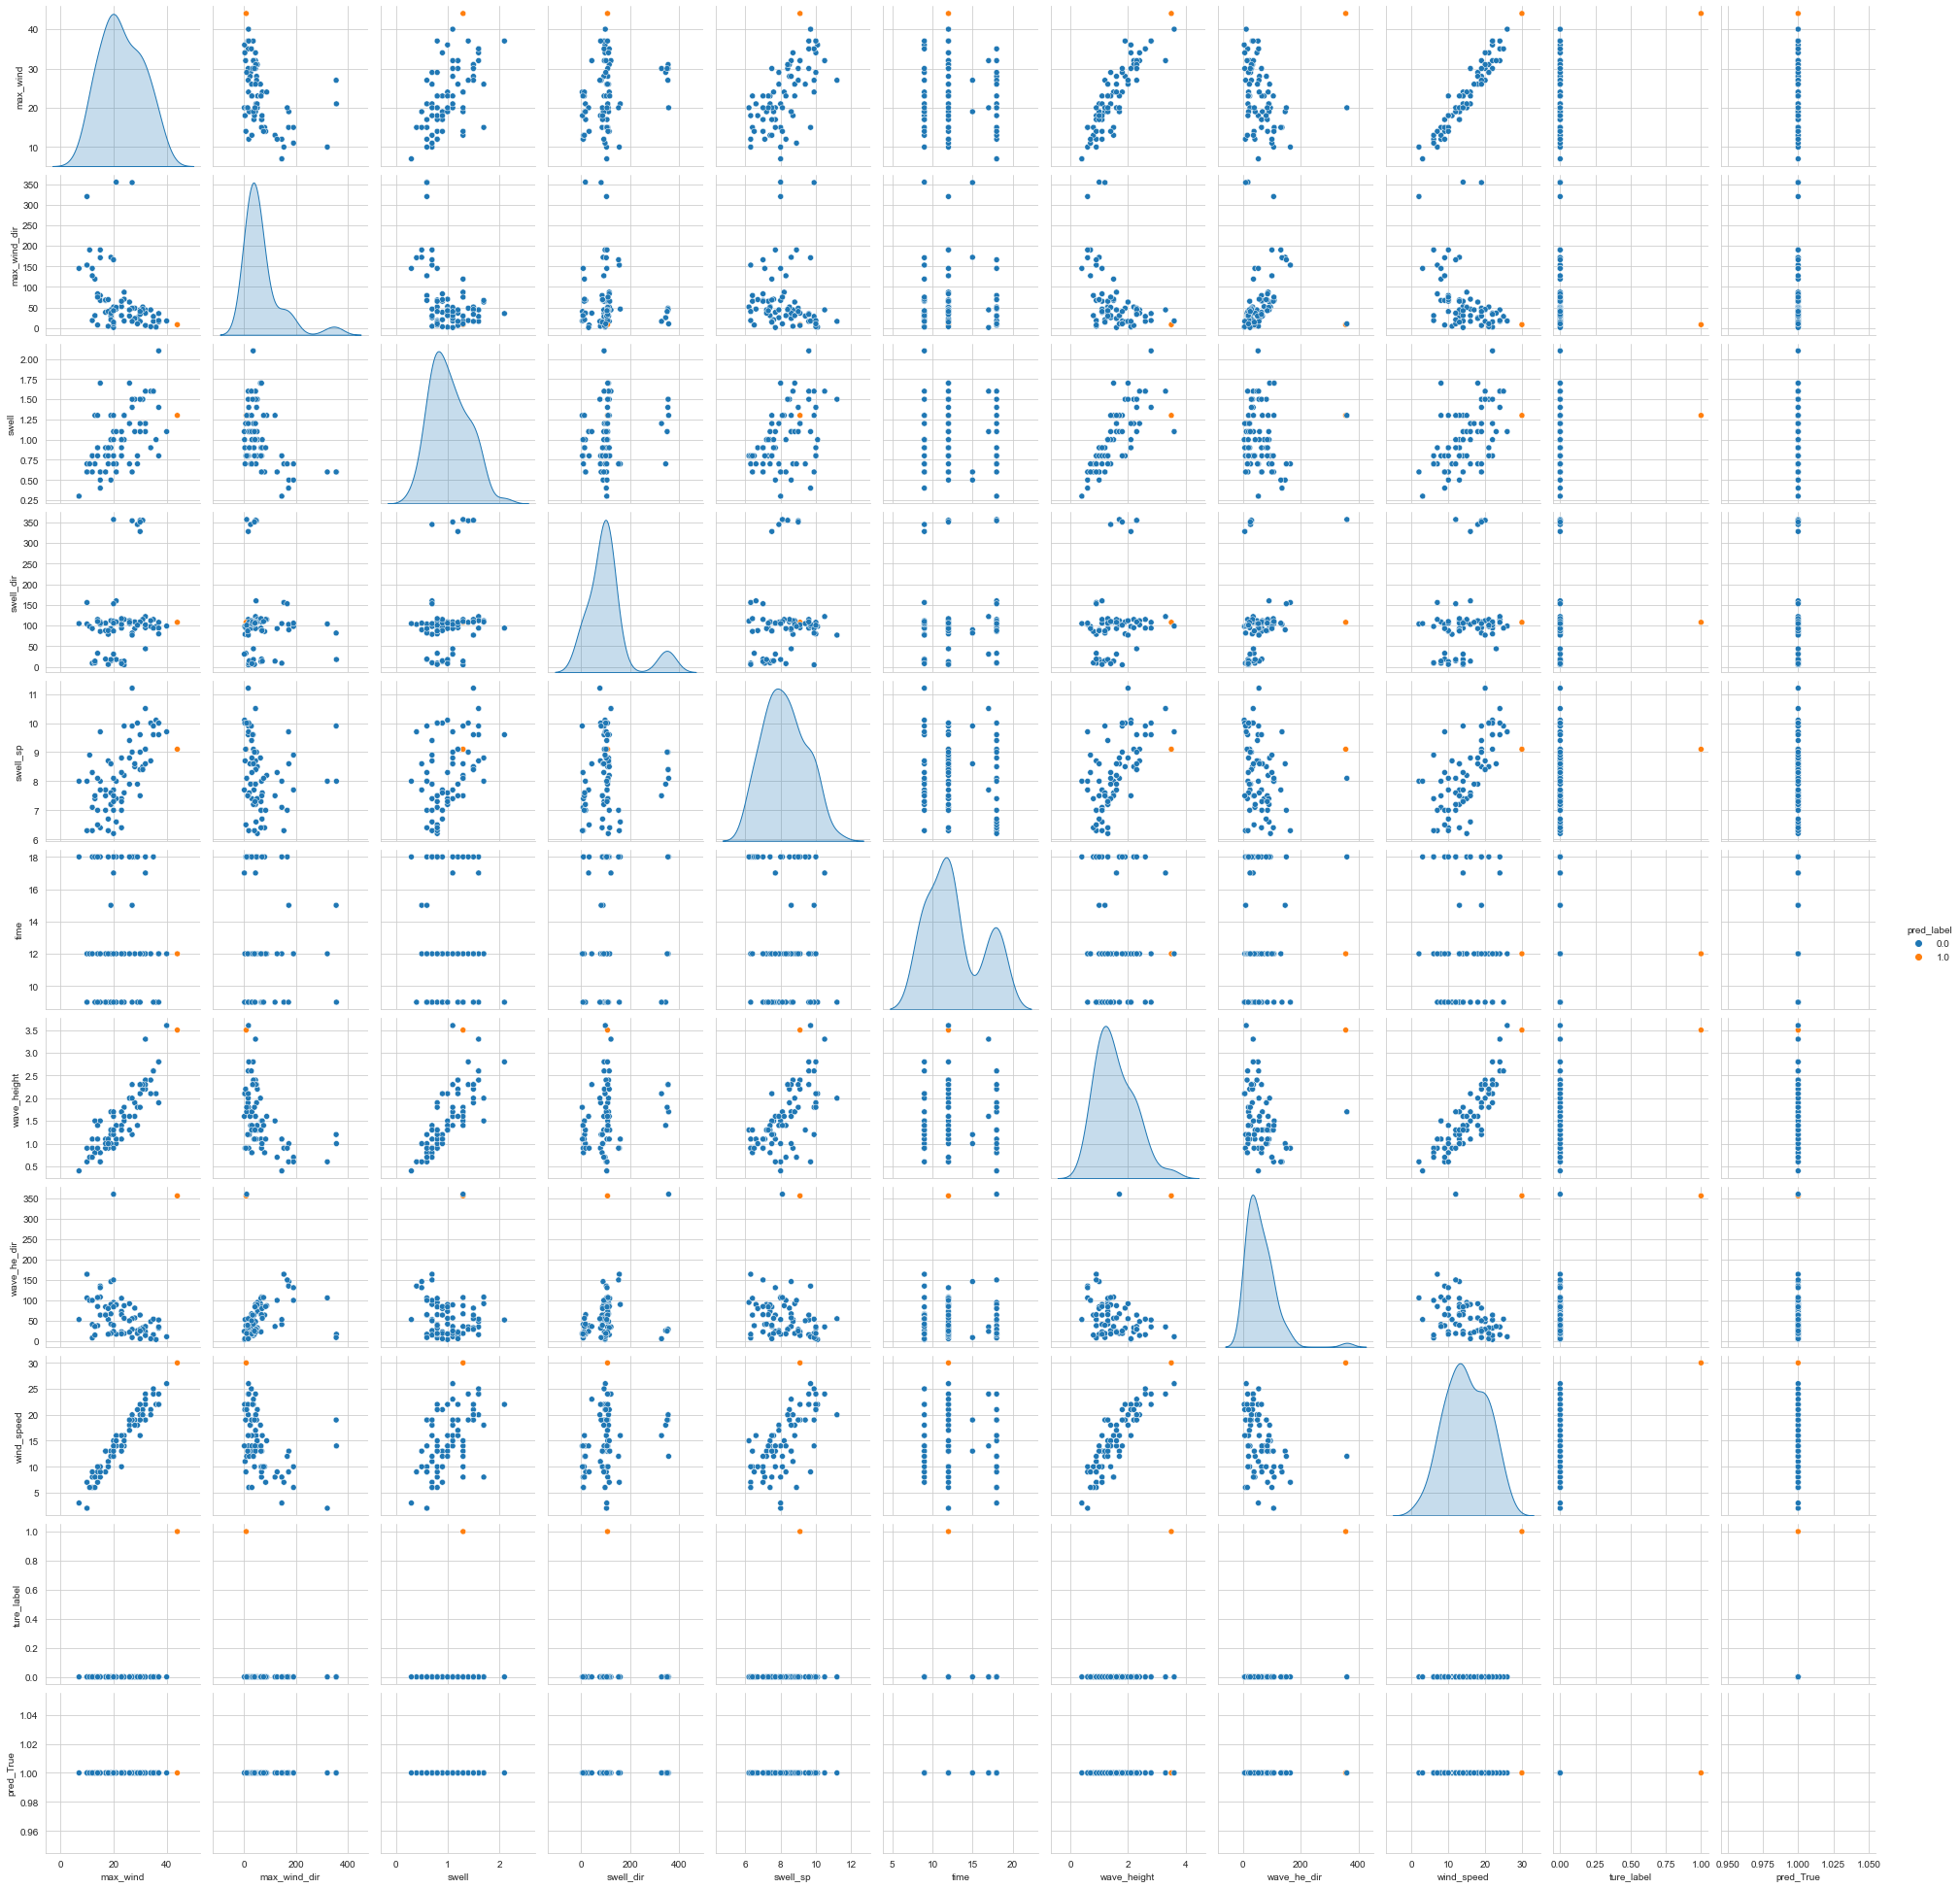
\includegraphics[keepaspectratio, scale=0.25]{fig/chapter4/kurosima_0_pred.png}
 \caption{黒島航路当日モデルの予測ラベル別}
 \label{kurosima_0_scatter_pred}
\end{figure}

\begin{figure}[H]
 \centering
 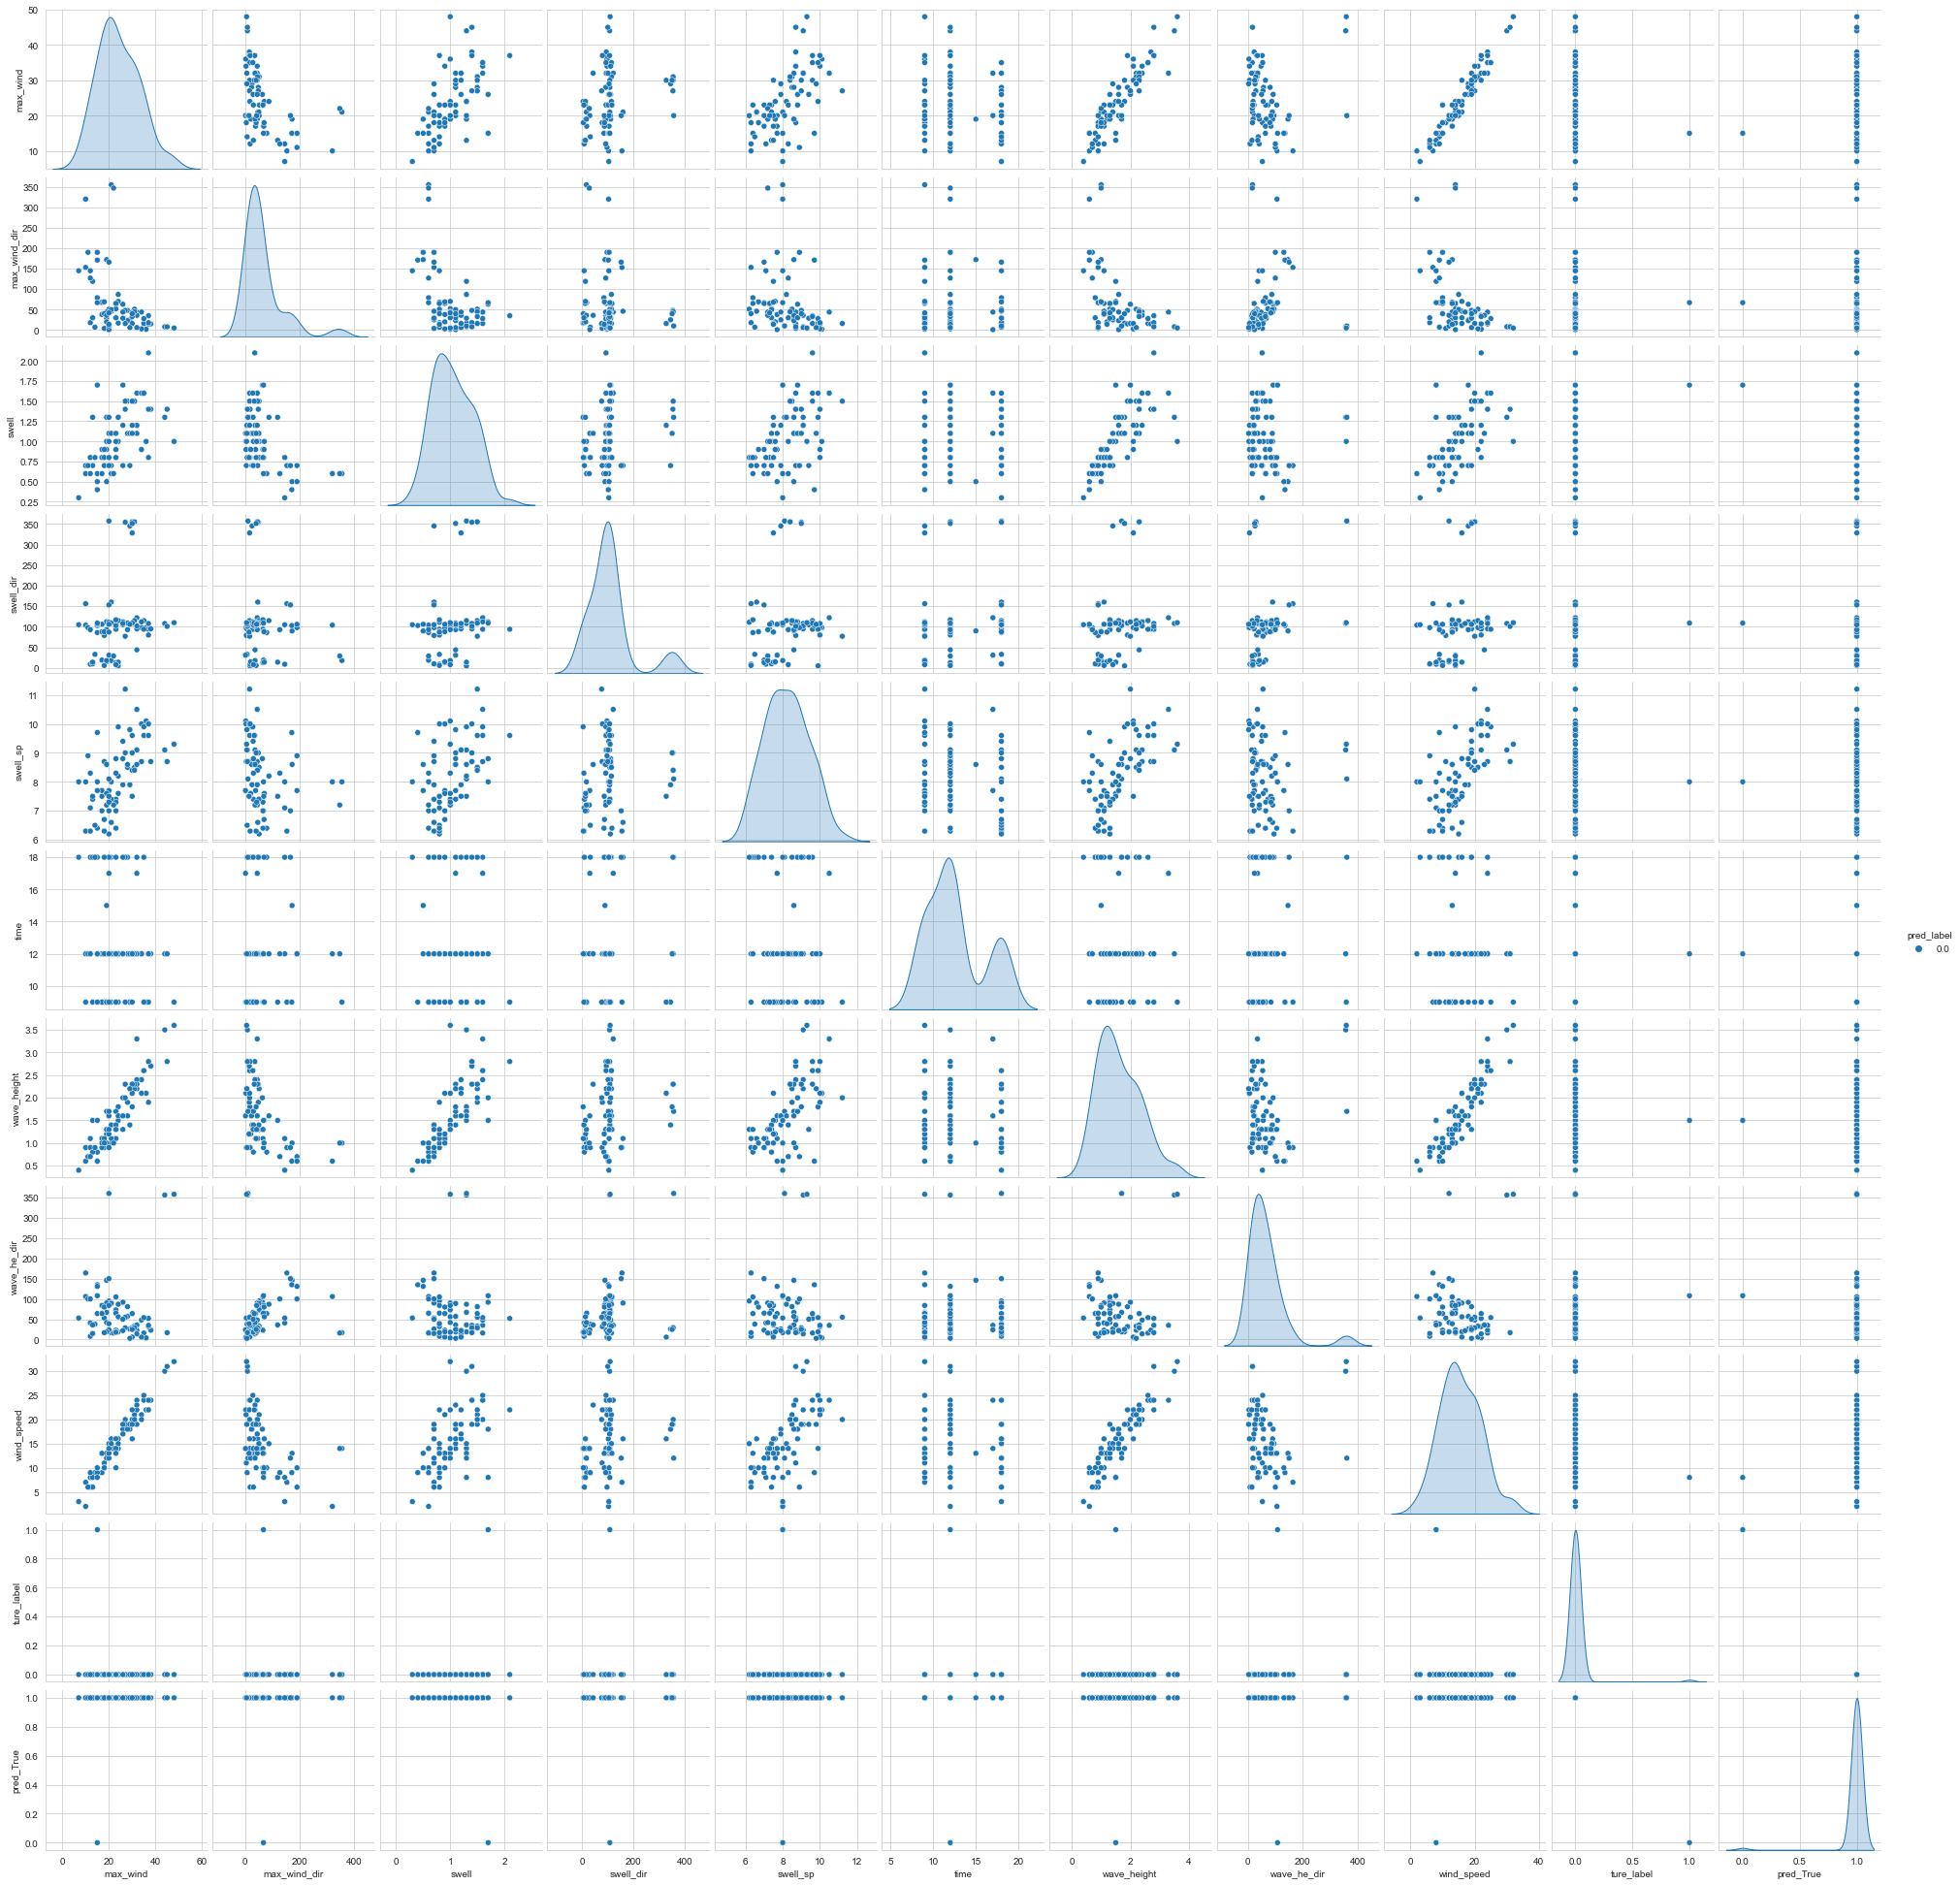
\includegraphics[keepaspectratio, scale=0.25]{fig/chapter4/kurosima_1_pred.png}
 \caption{黒島航路1日前モデルの予測ラベル別}
 \label{kurosima_1_scatter_pred}
\end{figure}

\begin{figure}[H]
 \centering
 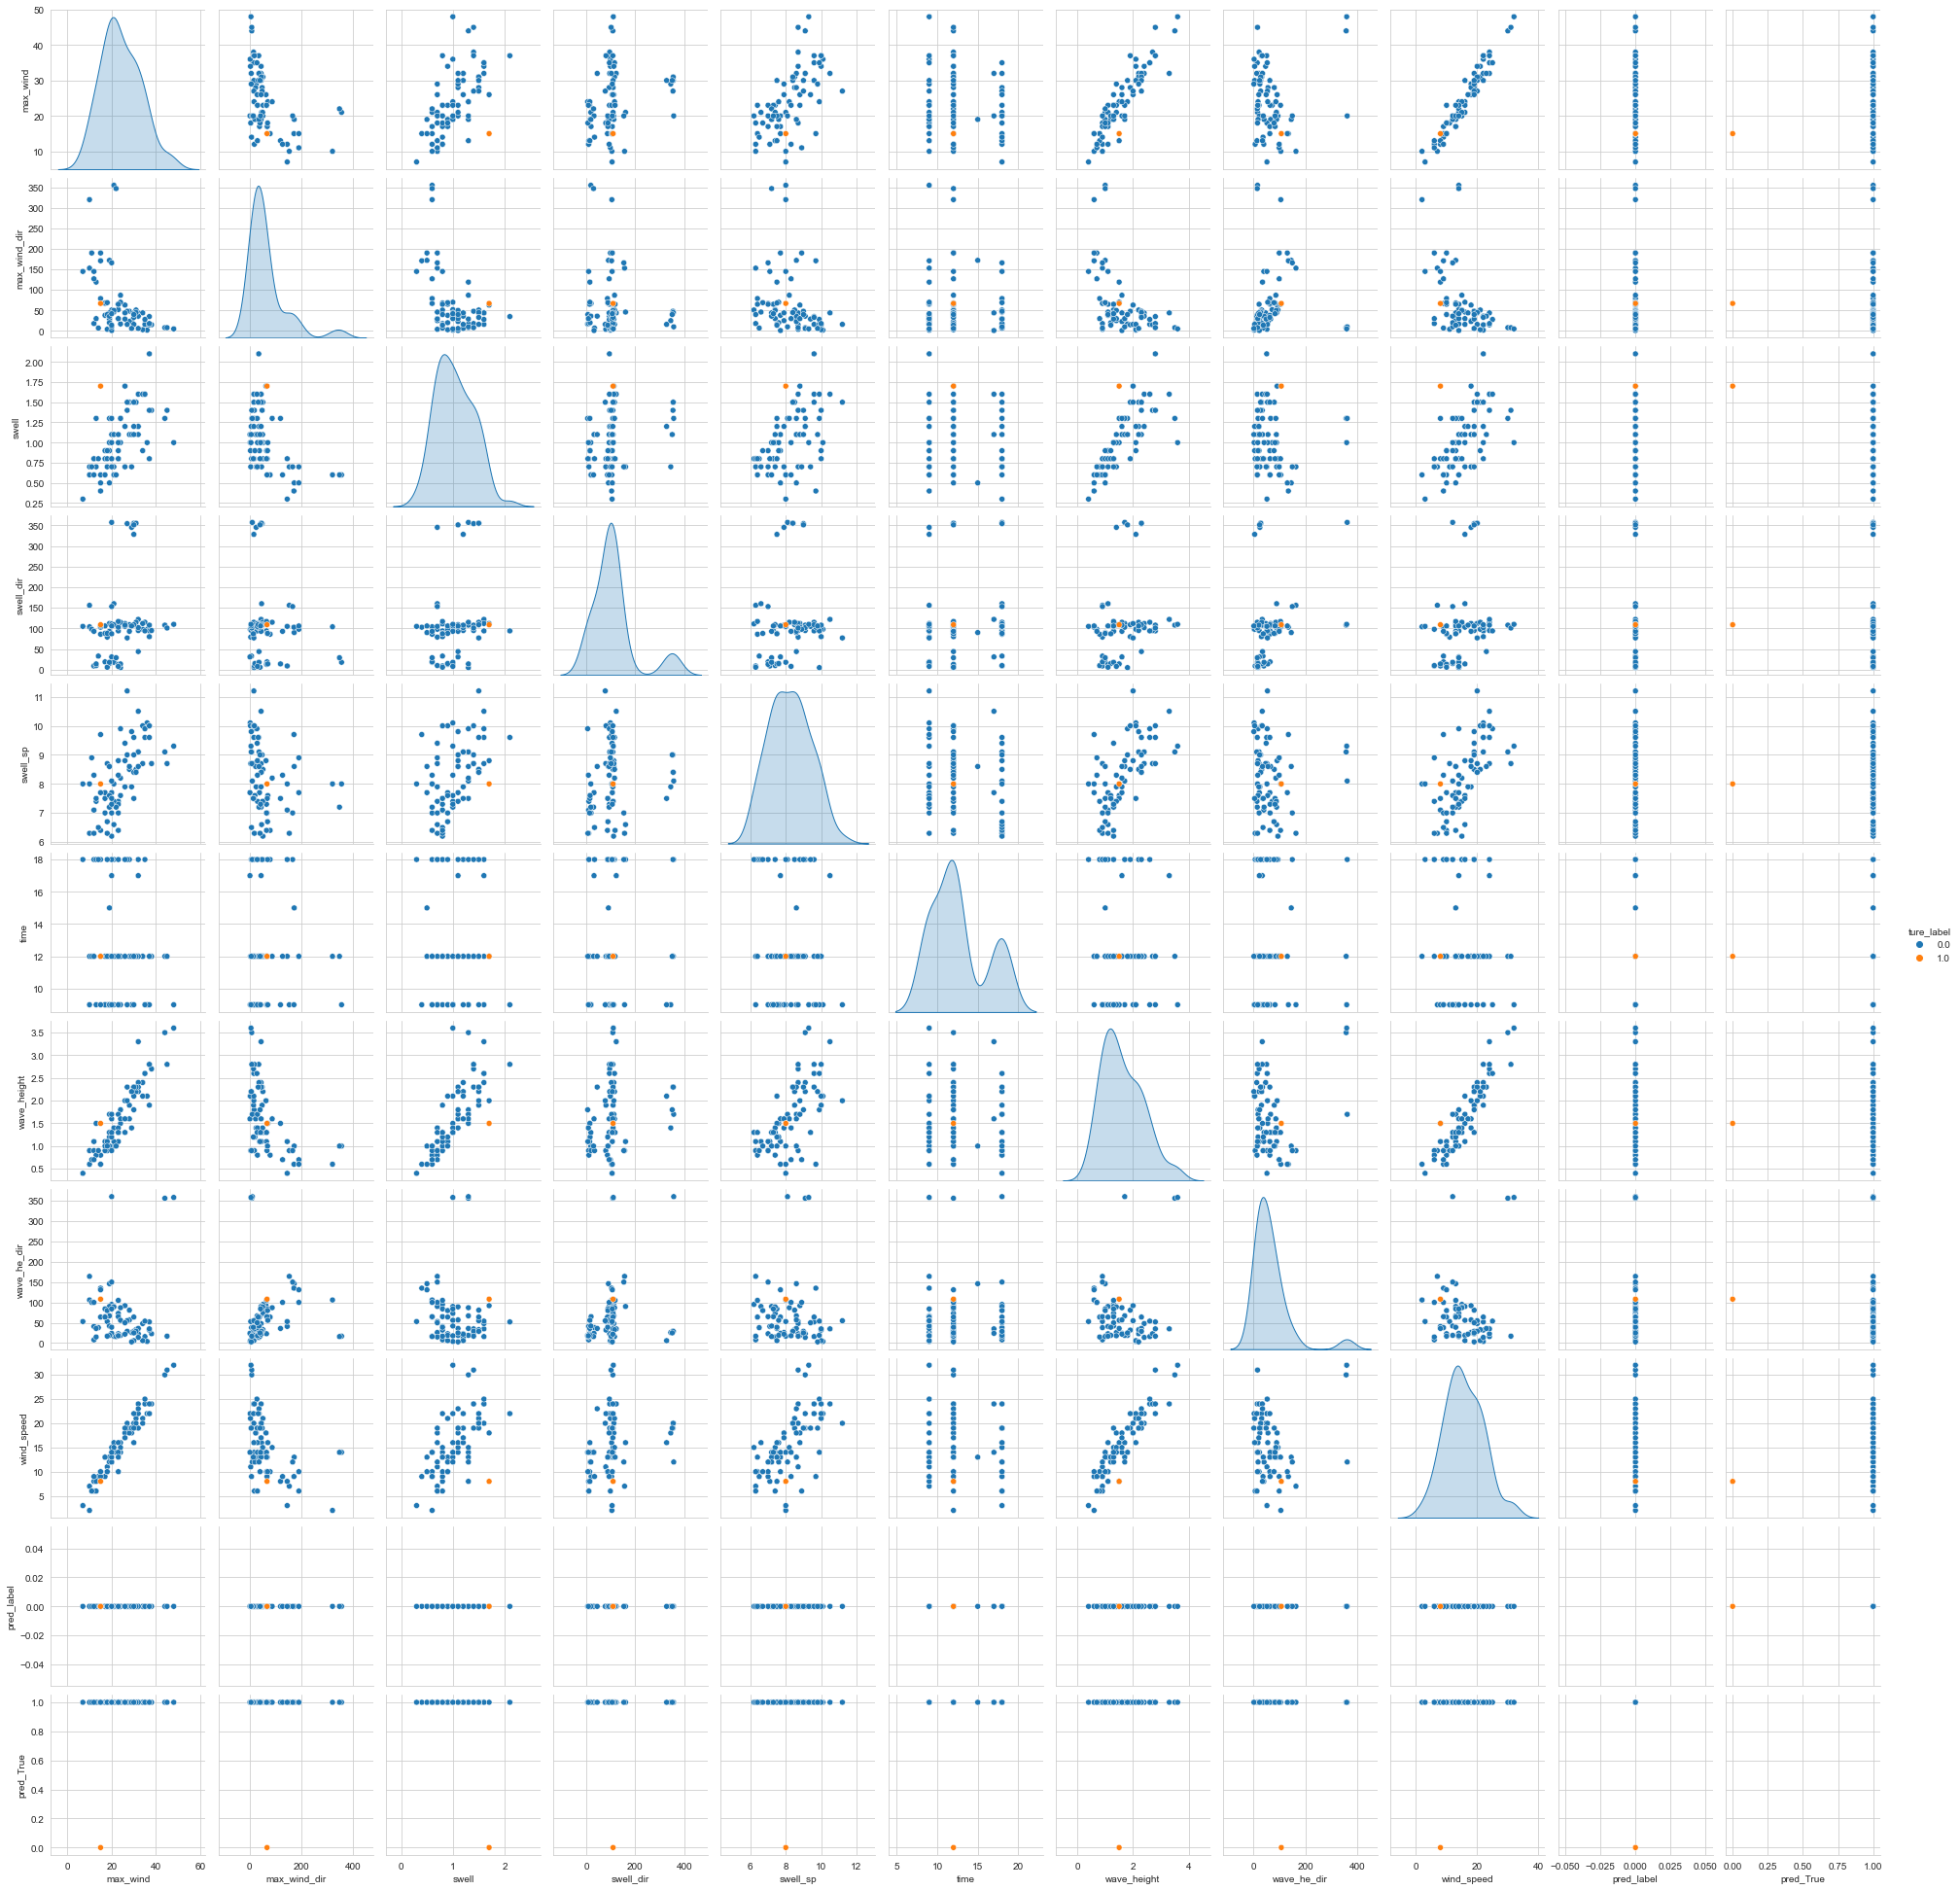
\includegraphics[keepaspectratio, scale=0.25]{fig/chapter4/kurosima_1_ture.png}
 \caption{黒島航路1日前モデルの真値ラベル別}
 \label{kurosima_1_scatter_ture}
\end{figure}

\subsection{画像データの考察}
\subsubsection{波高レイヤー画像}

表\ref{img_wave_hateruma}の波照間航路1日前モデルにおいてテストデータ予測結果の混同行列図\ref{hateruma_1_conf}となり、True labelの0は運航、1が欠航であり、Predicted labelは予想したラベルとなる。TP、FN、FP、TNの画像例として図\ref{hateruma_1_TP}、図\ref{hateruma_1_FN}、図\ref{hateruma_1_FP}、図\ref{hateruma_1_TN}がある。これらの画像からこのモデルは画像全体が青色の場合に運航と判断していることが確認できる。またその反対に画像全体と画像中心部が赤色の画像を欠航と判断していることが確認できる。FP部分の画像が運航として分類された理由として
、図\ref{hateruma_1_FP}の画像は12月24日13:00に取得された画像だが教師ラベル1日後の12月25日13:00のデータが紐づいているため12月25日13:00の画像を確認すると図\ref{hateruma_1_FP_1}となっており波照間航路線のある部分は青色が確認できる。そのため当日は運航していたと考えられ、図\ref{hateruma_1_FP}の画像の波照間航路線は赤色になっており欠航とモデルは判断したと考えられる。FN部分の画像で運航されると誤分類されているのは図\ref{hateruma_1_FN}の一枚のみであった。この画像の教師ラベル当日の時間の画像を見ると図\ref{hateruma_1_FN_1}となっており、画像は波照間行路線の部分が青色のため当日は運航でき、教師データは運航となっている。しかし、画像大部分が赤色なのでモデルは欠航と予測したと考えられる。

\begin{figure}[H]
 \centering
 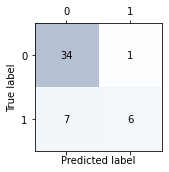
\includegraphics[keepaspectratio, scale=0.8]{fig/chapter4/wave_hateruma_1/hateruma_1_conf.png}
 \caption{波照間航路1日前モデルの混同行列}
 \label{hateruma_1_conf}
\end{figure}

\newpage

\begin{figure}[htbp]
 \begin{minipage}{0.5\hsize}
  \begin{center}
   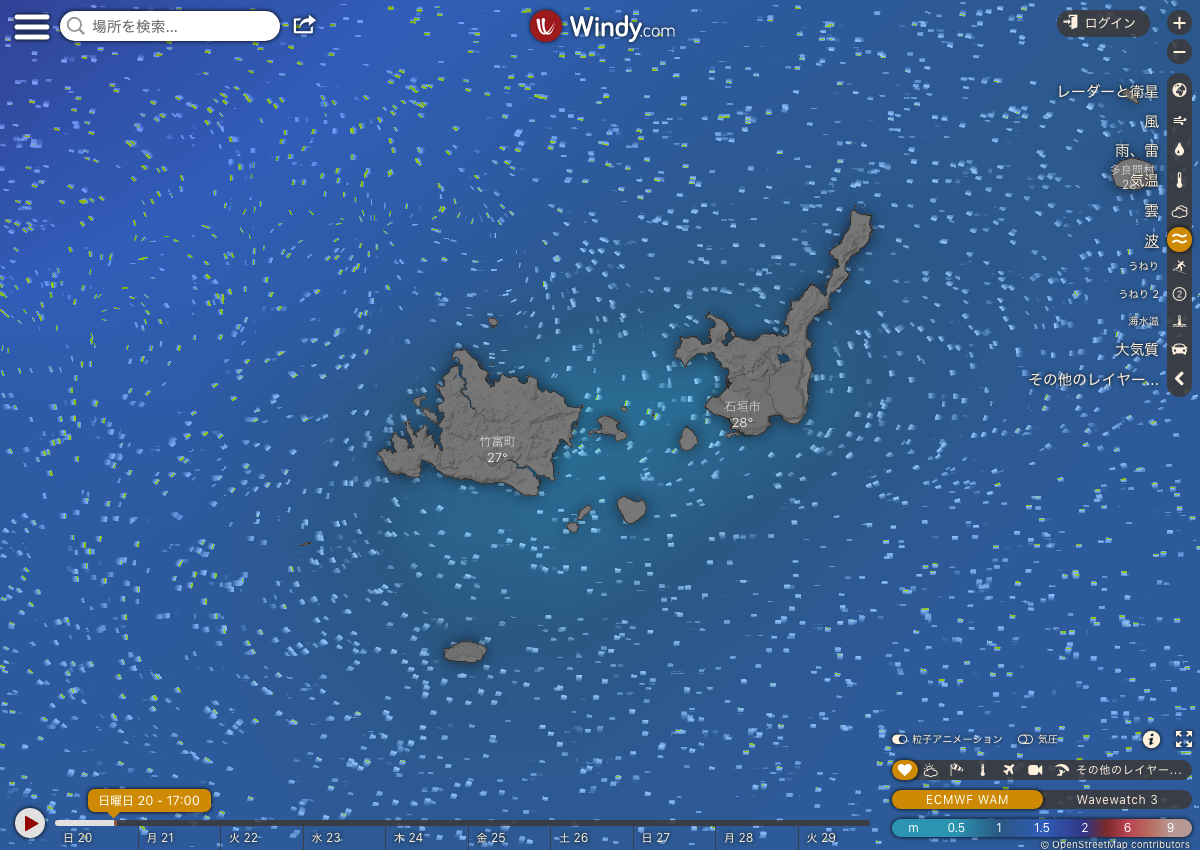
\includegraphics[keepaspectratio, scale=0.16]{fig/chapter4/wave_hateruma_1/TP.png}
   %2020-09-20_17/00_0_0.png
  \end{center}
  \caption{波照間航路1日前モデルのTP画像例}
  \label{hateruma_1_TP}
 \end{minipage}
 \begin{minipage}{0.5\hsize}
  \begin{center}
  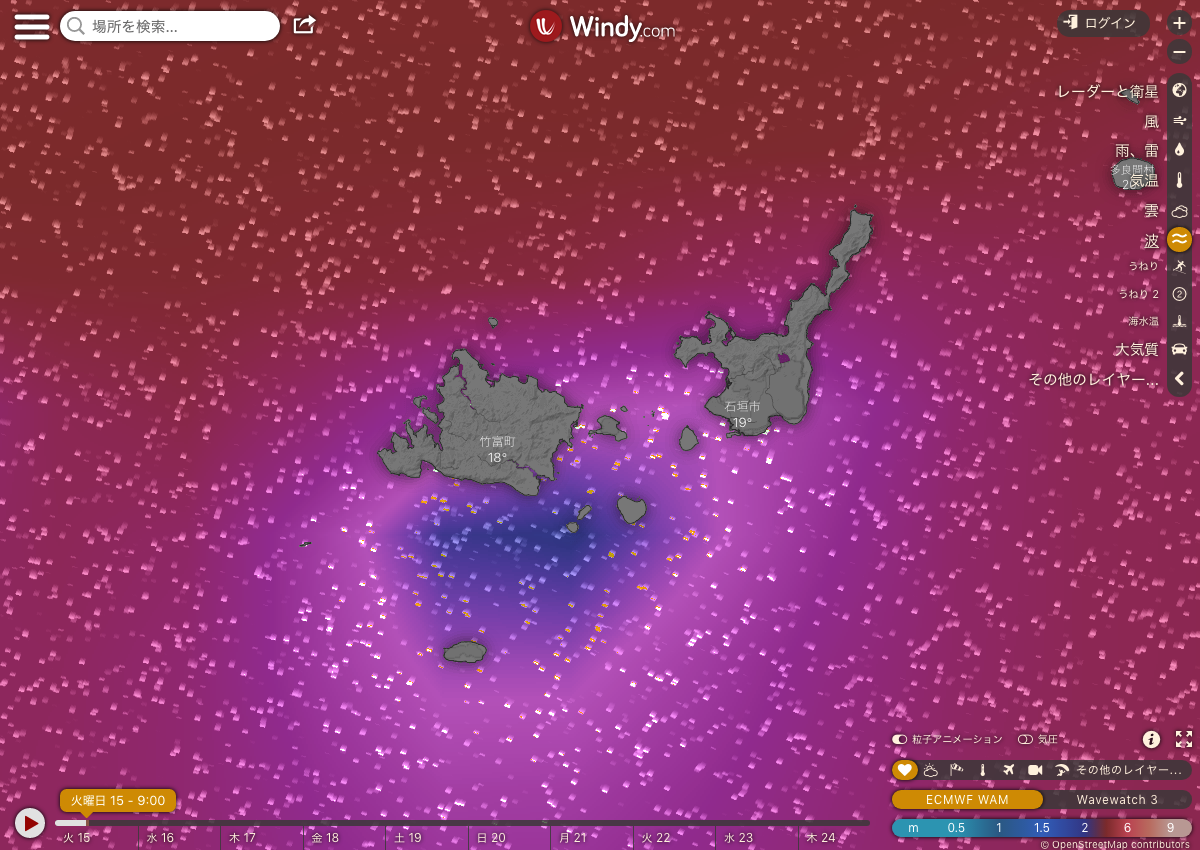
\includegraphics[keepaspectratio, scale=0.16]{fig/chapter4/wave_hateruma_1/FN.png}
  %2020-12-15 9/00_1_0
  \end{center}
   \caption{波照間航路1日前モデルのFN画像}
  \label{hateruma_1_FN}
 \end{minipage}
\end{figure}

\begin{figure}[htbp]
 \begin{minipage}{0.5\hsize}
  \begin{center}
   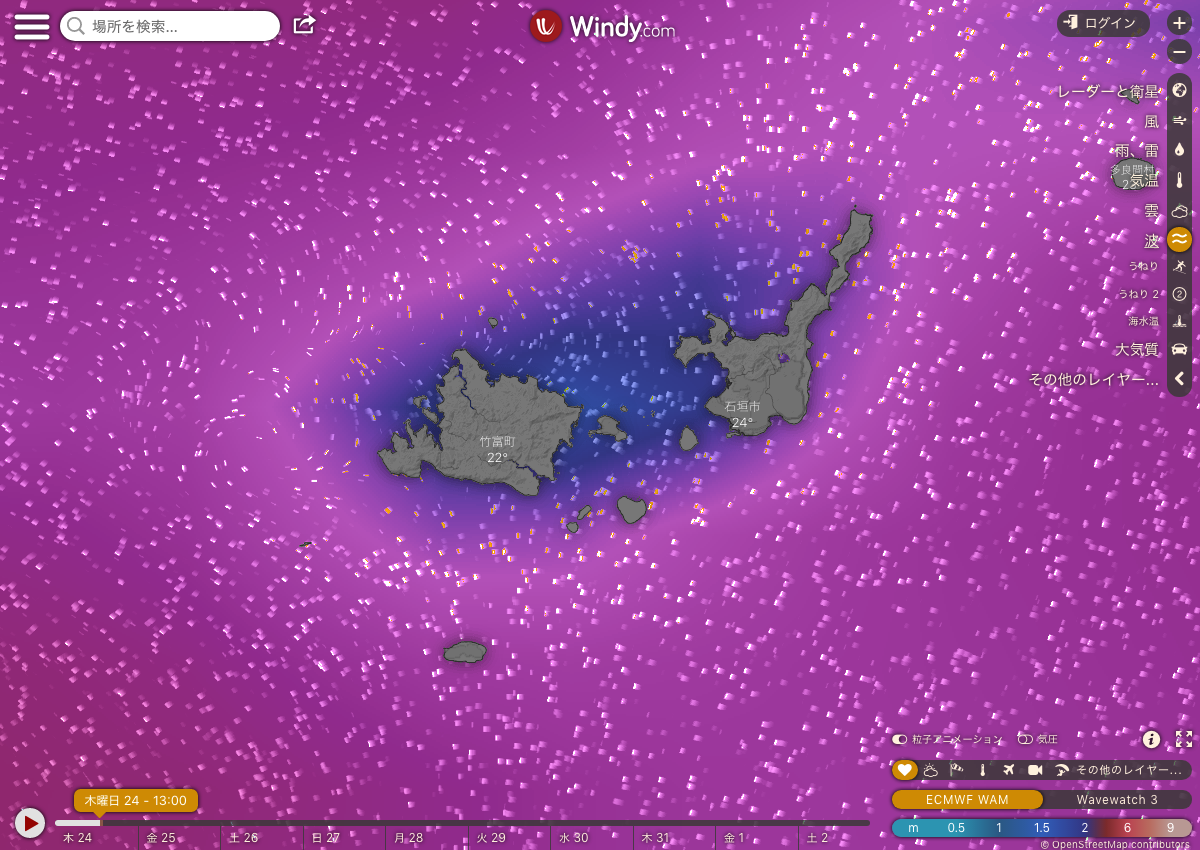
\includegraphics[keepaspectratio, scale=0.16]{fig/chapter4/wave_hateruma_1/FP.png}
   %2020-12-24 13/00/00
  \end{center}
  \caption{波照間航路1日前モデルのFP画像例}
  \label{hateruma_1_FP}
 \end{minipage}
 \begin{minipage}{0.5\hsize}
  \begin{center}
  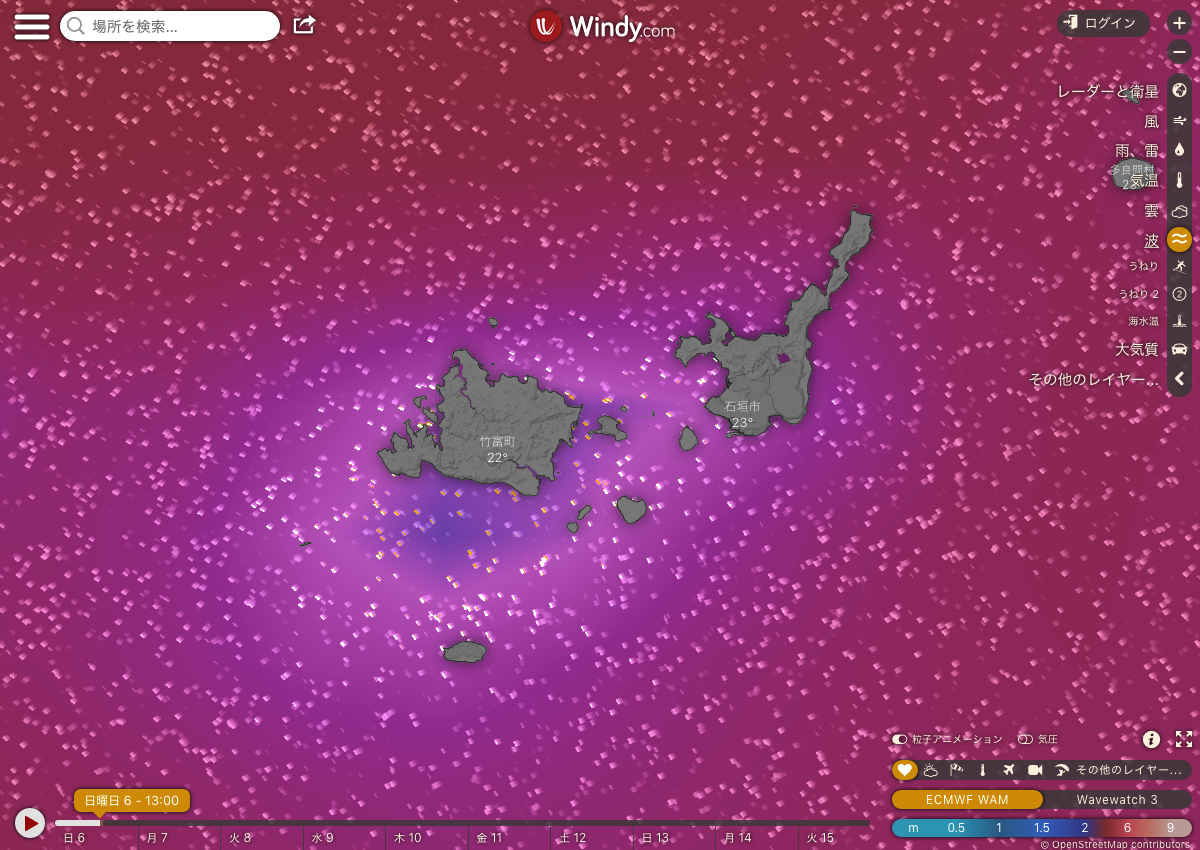
\includegraphics[keepaspectratio, scale=0.16]{fig/chapter4/wave_hateruma_1/TN.png}
  %2021-12-06 13/00_1_1.png
  \end{center}
   \caption{波照間航路1日前モデルのTN画像例}
  \label{hateruma_1_TN}
 \end{minipage}
\end{figure}

\begin{figure}[H]
 \begin{minipage}{0.5\hsize}
  \begin{center}
   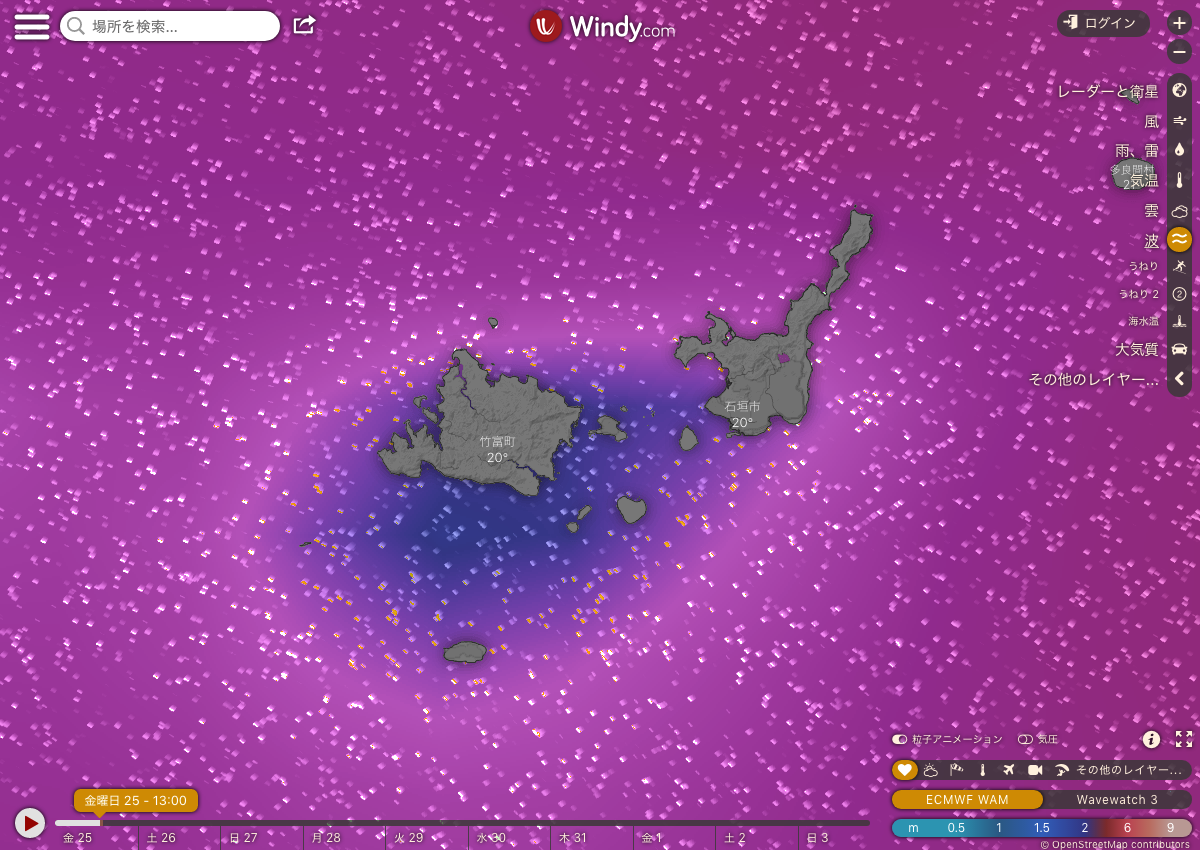
\includegraphics[keepaspectratio, scale=0.16]{fig/chapter4/wave_hateruma_1/FP_1.png}
   %2020-12-24 13/00/00
  \end{center}
  \caption{FP画像1日後の教師ラベル当日の画像}
  \label{hateruma_1_FP_1}
 \end{minipage}
 \begin{minipage}{0.5\hsize}
  \begin{center}
  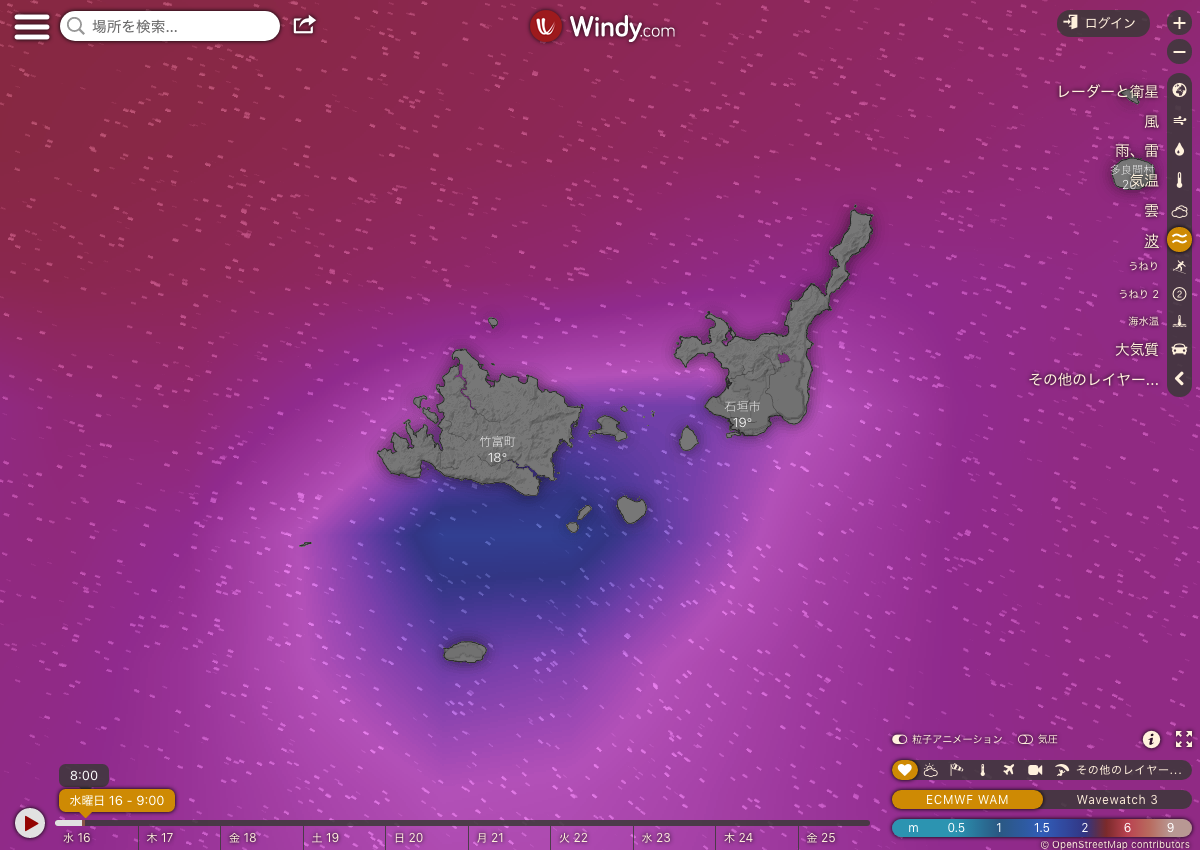
\includegraphics[keepaspectratio, scale=0.16]{fig/chapter4/wave_hateruma_1/FN_1.png}
  %2021-12-06 13/00_1_1.png
  \end{center}
   \caption{FN画像1日後の教師ラベル当日の画像}
  \label{hateruma_1_FN_1}
 \end{minipage}
\end{figure}

\newpage

表\ref{img_wave_hateruma}の波照間航路2日前モデルにおいてテストデータ予測結果の混同行列図\ref{hateruma_2_conf}となり、モデルが運航どのテストデータに対しても運航であると予測していることが確認できる。トレーニングデータを確認すると運航ラベルの付いた画像に図\ref{aka}のような画像や図\ref{unkou_ao}があることが確認できた。トレーニングデータ中の運航ラベルのついたデータが画像によって一貫性がなく、RGBの値も大きく異なるためにモデルの学習が適切に行えていないことが考えられる。%また、この航路は時間が進むに連れて教師データのが激しいため、3日前モデル以降のモデルでは全く予測できないことが考えられる。

%0 0 2021-01-01 09:50:00 ../data/now_img_scrape/wave_height/9:00/2020-12-30 09:00:00.png
%0 0 2020-09-13 13:25:00 ../data/now_img_scrape/wave_height/13:00/2020-09-1113:00:00.png

\begin{figure}[H]
 \centering
 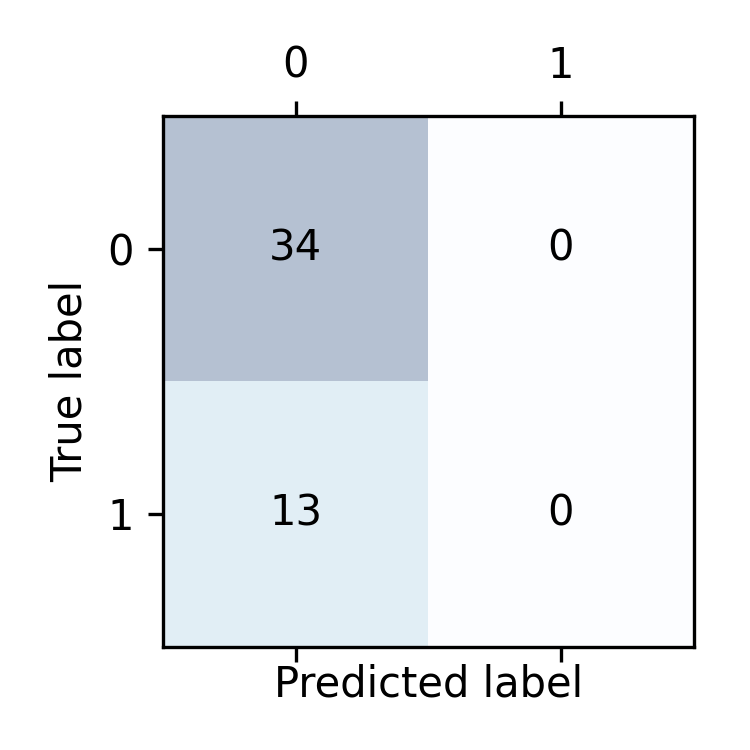
\includegraphics[keepaspectratio, scale=0.8]{fig/chapter4/wave_hateruma_2/hateruma_route_hateruma_dep_2.png}
 \caption{波照間航路2日前モデルの混同行列}
 \label{hateruma_2_conf}
\end{figure}

\begin{figure}[htbp]
 \begin{minipage}{0.5\hsize}
  \begin{center}
   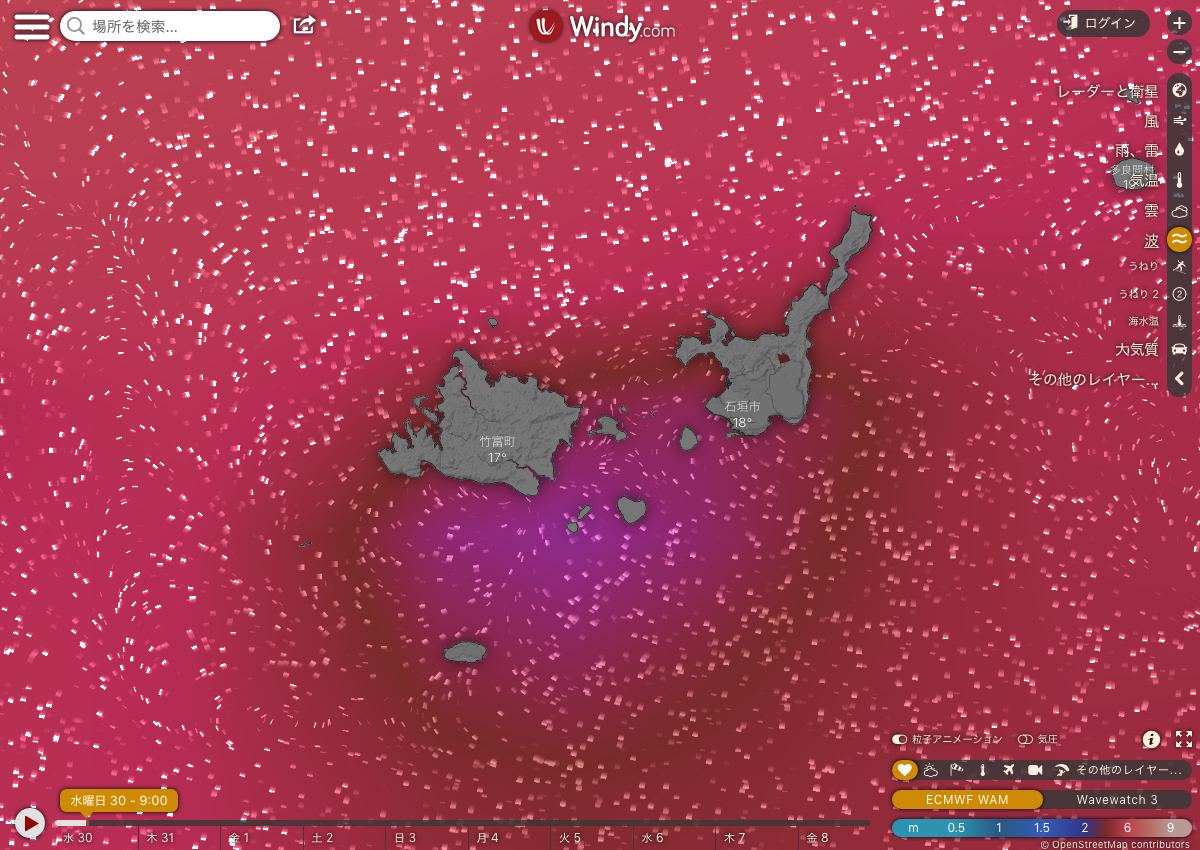
\includegraphics[keepaspectratio, scale=0.17]{fig/chapter4/wave_hateruma_2/unkou_aka.png}
   %2020-12-24 13/00/00
  \end{center}
  \caption{教師ラベル:運航 1}
  \label{aka}
 \end{minipage}
 \begin{minipage}{0.5\hsize}
  \begin{center}
  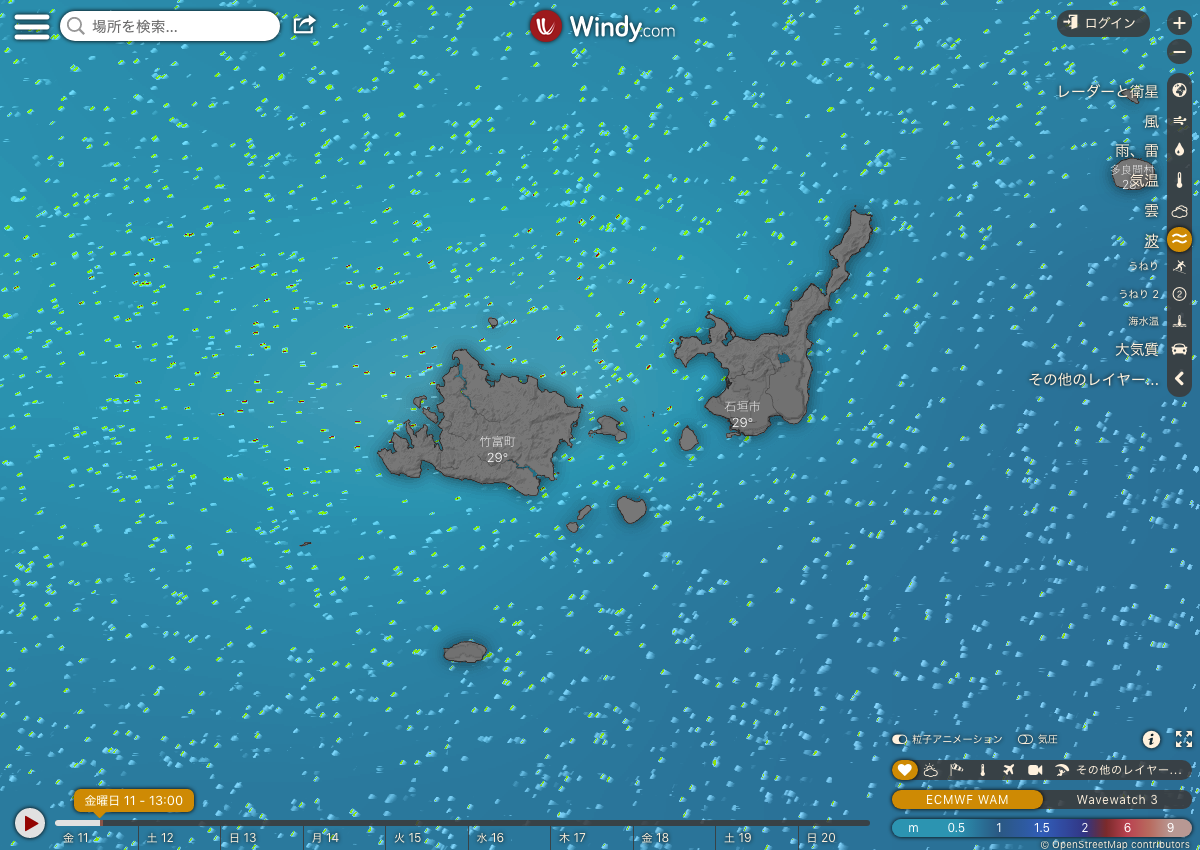
\includegraphics[keepaspectratio, scale=0.17]{fig/chapter4/wave_hateruma_2/unkou_ao.png}
  %2021-12-06 13/00_1_1.png
  \end{center}
   \caption{教師ラベル:運航 2}
  \label{unkou_ao}
 \end{minipage}
\end{figure}

表\ref{img_wave_hatoma}の波照間航路当日モデルにおいてテストデータ予測結果の混同行列図\ref{hatoma_0_conf}となり、TP、FN、FP、TNの画像例として図\ref{hatoma_0_TP}、図\ref{hatoma_0_FN}、図\ref{hatoma_0_FP}、図\ref{hatoma_0_TN}がある。FNが誤分類された理由としてトレーニングデータ中の画像として図\ref{hatoma_0_FN_setu}があり、図\ref{hatoma_0_FN}と傾向が似ているにもかかわらず教師データが欠航のため、誤分類されたと考えられる。また、傾向が似ているにもかかわらず教師データが異なる理由として、当日の状況が視程が500m以下\cite{stan}であったと考えられる。または、風速レイヤーの画像を確認すると風向きが真逆だったため、風向が原因であると考えられる。FPが誤分類された理由として、トレーニングデータ中の画像に図\ref{hatoma_0_FP_setu}が教師データが運航として学習されているために傾向の似ている図\ref{hatoma_0_FP}が誤分類されたと考えられる。
\\ モデルがn日前のnが増加するたびにF値が減少していることが確認できる。これは教師データと特徴量のデータを取得した日付が離れることに比例していると考えられる。

\begin{figure}[H]
 \centering
 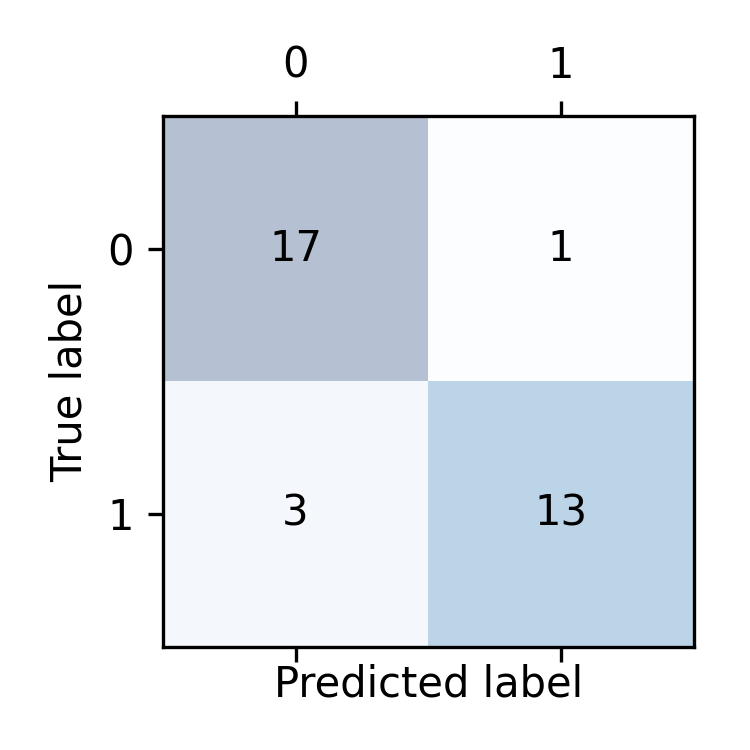
\includegraphics[keepaspectratio, scale=0.8]{fig/chapter4/wave_hatoma_0/hatoma_route_hatoma_dep_0.png}
 \caption{鳩間島航路当日モデルの混同行列}
 \label{hatoma_0_conf}
\end{figure}

\begin{figure}[htbp]
 \begin{minipage}{0.5\hsize}
  \begin{center}
   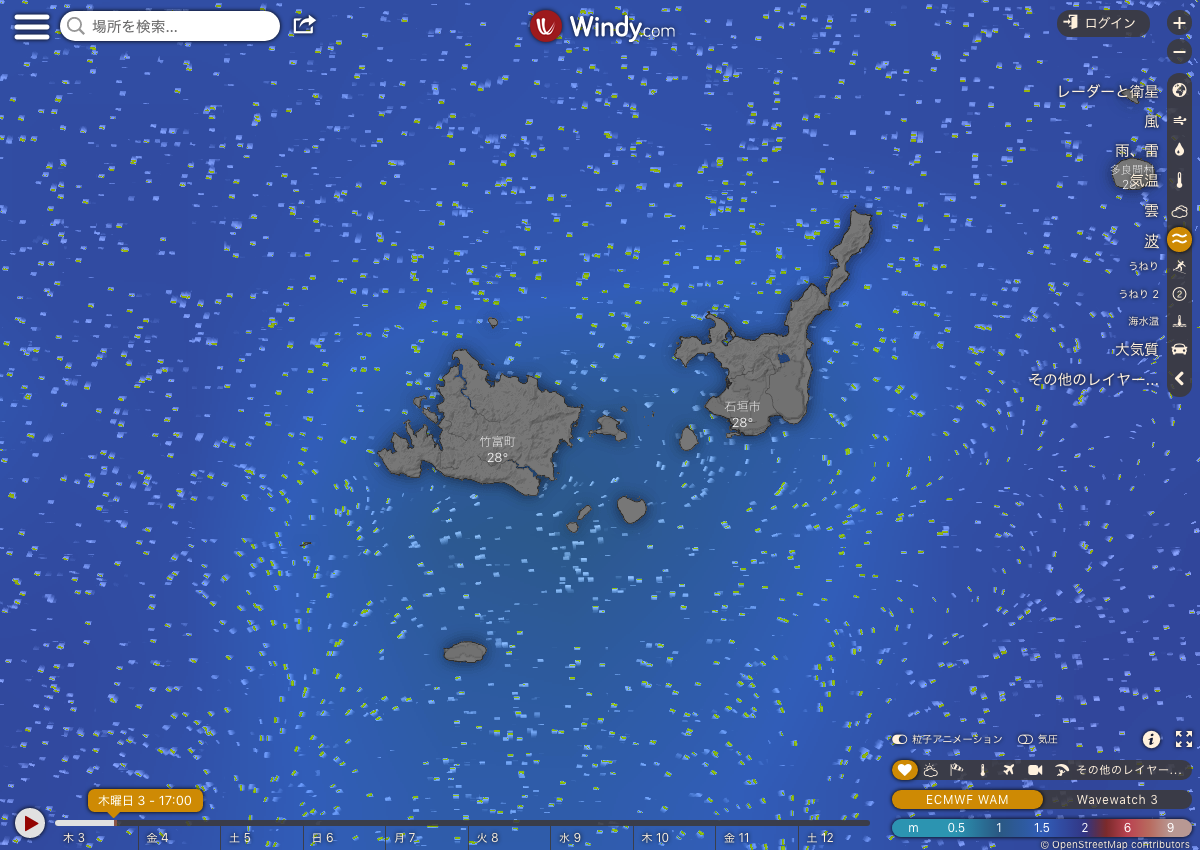
\includegraphics[keepaspectratio, scale=0.16]{fig/chapter4/wave_hatoma_0/TP.png}
   %2020-09-03 17/00/00_0_0
  \end{center}
  \caption{鳩間島航路当日モデルのTP画像例}
  \label{hatoma_0_TP}
 \end{minipage}
 \begin{minipage}{0.5\hsize}
  \begin{center}
  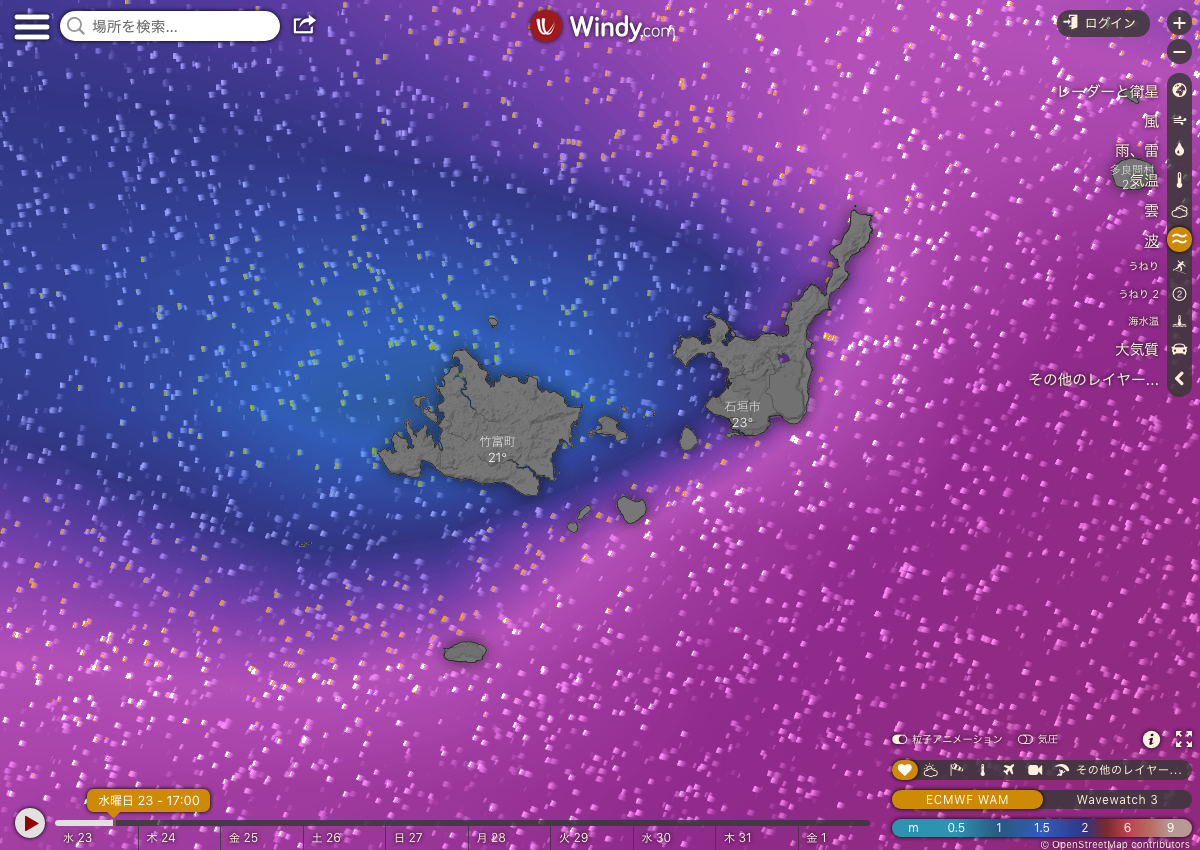
\includegraphics[keepaspectratio, scale=0.16]{fig/chapter4/wave_hatoma_0/FN.png}
   %2020-12-23 17/00/00.png
  \end{center}
   \caption{鳩間島航路当日モデルのFN画像}
  \label{hatoma_0_FN}
 \end{minipage}
\end{figure}

\begin{figure}[htbp]
 \begin{minipage}{0.5\hsize}
  \begin{center}
   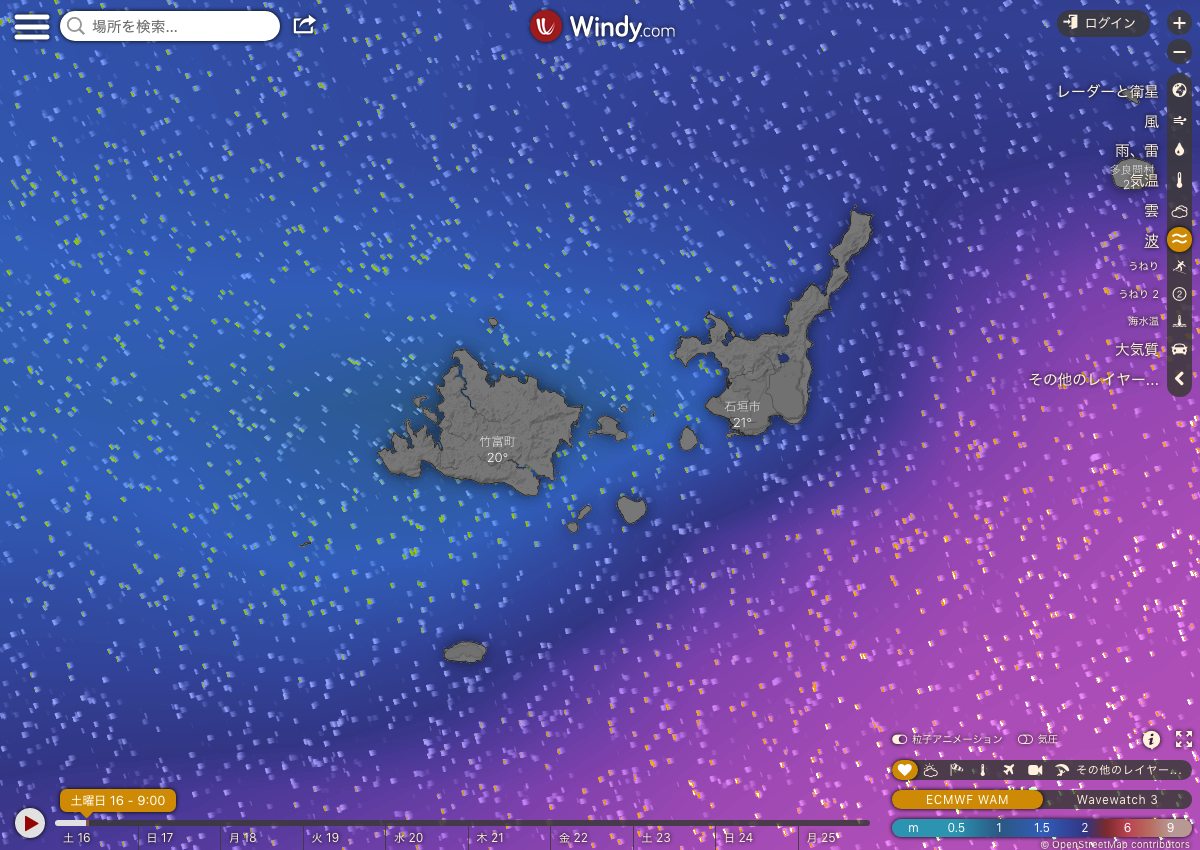
\includegraphics[keepaspectratio, scale=0.16]{fig/chapter4/wave_hatoma_0/FP.png}
   %2021-01-16 09/00/00_1_0.png
  \end{center}
  \caption{鳩間島航路当日モデルのFP画像例}
  \label{hatoma_0_FP}
 \end{minipage}
 \begin{minipage}{0.5\hsize}
  \begin{center}
  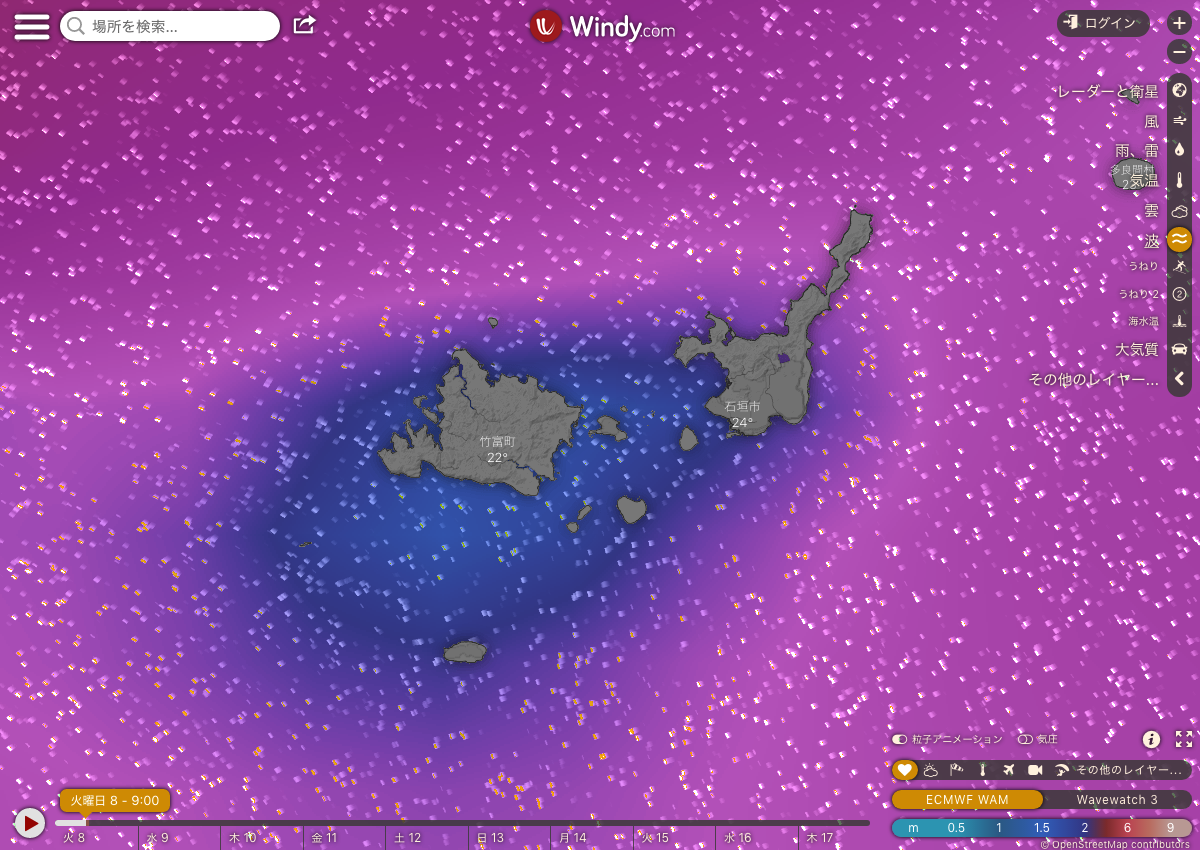
\includegraphics[keepaspectratio, scale=0.16]{fig/chapter4/wave_hatoma_0/TN.png}
  %2020-12-08 09/00/00_1_1.png
  \end{center}
   \caption{鳩間島航路当日モデルのTN画像例}
  \label{hatoma_0_TN}
 \end{minipage}
\end{figure}

\begin{figure}[H]
 \begin{minipage}{0.5\hsize}
  \begin{center}
   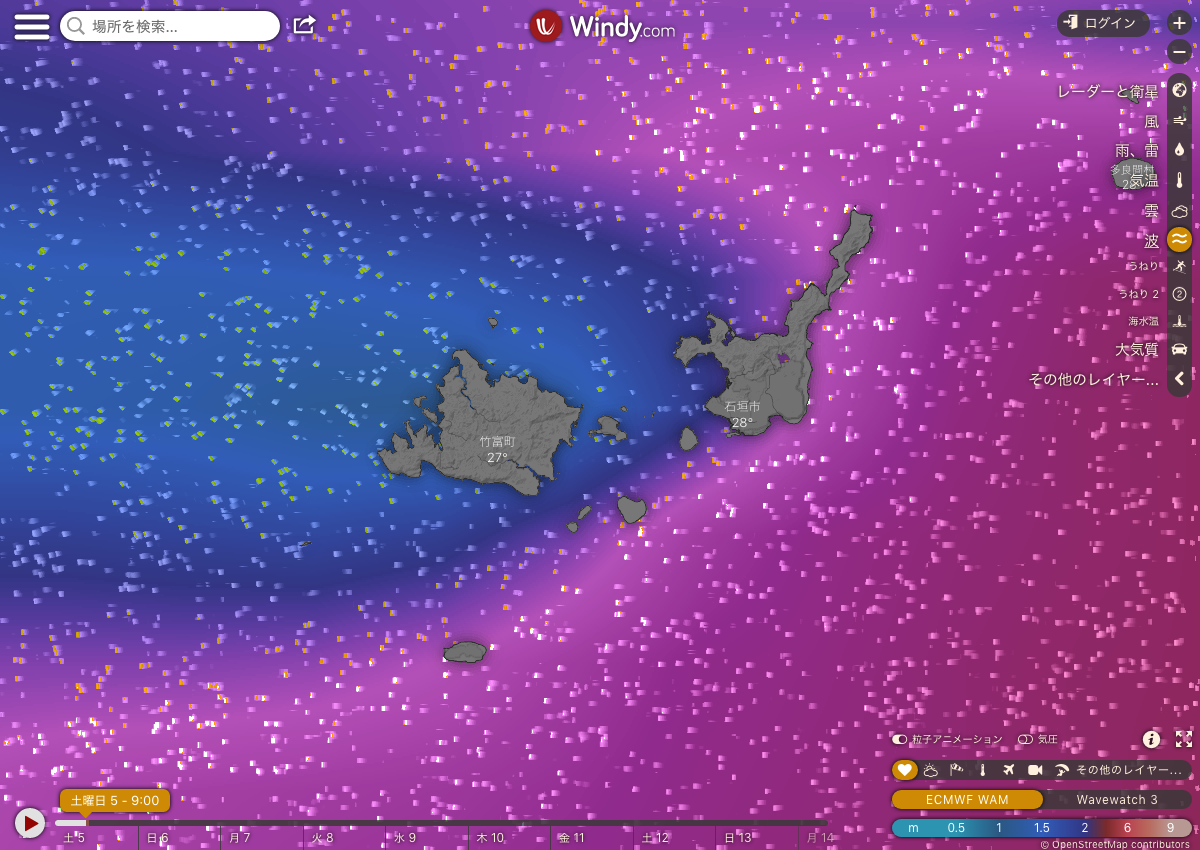
\includegraphics[keepaspectratio, scale=0.16]{fig/chapter4/wave_hatoma_0/FN_setu.png}
   %2020-09-05 09/00/00_FN_setu.png
  \end{center}
  \caption{教師ラベル:欠航}
  \label{hatoma_0_FN_setu}
 \end{minipage}
 \begin{minipage}{0.5\hsize}
  \begin{center}
  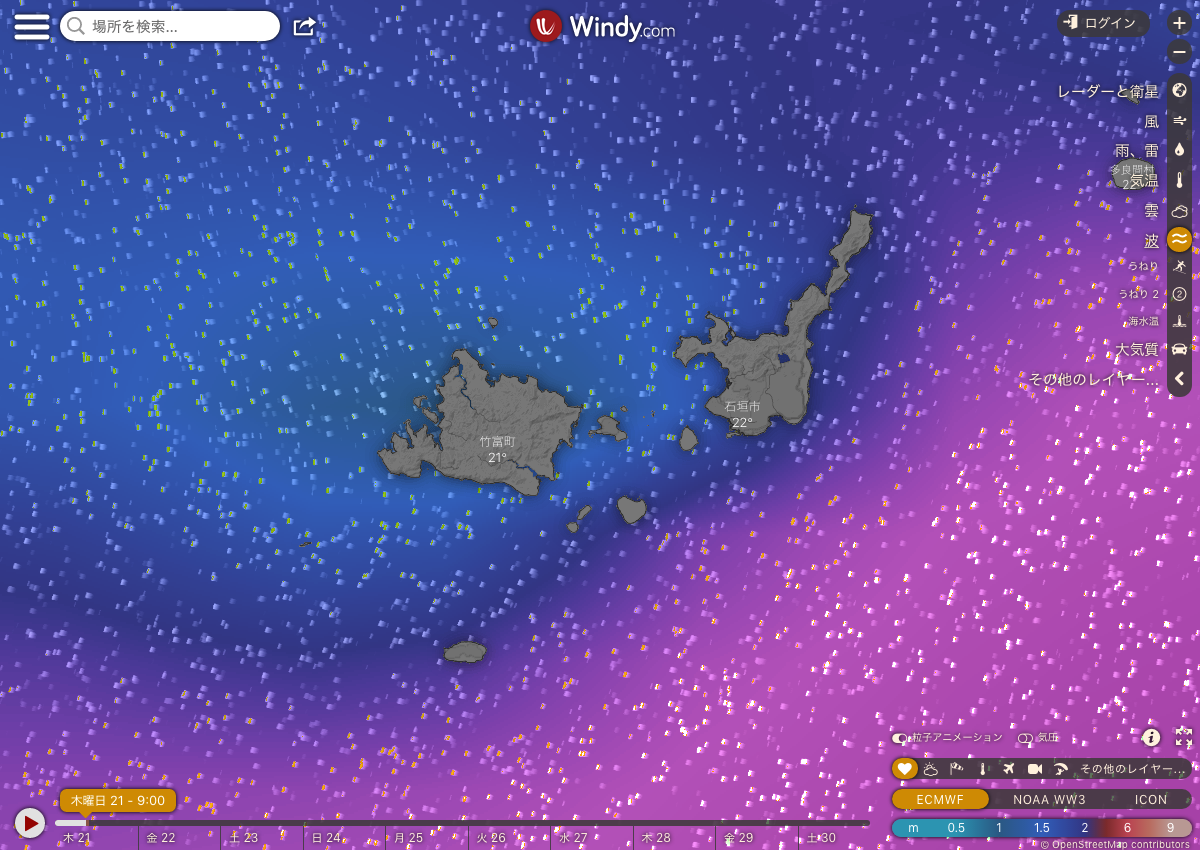
\includegraphics[keepaspectratio, scale=0.16]{fig/chapter4/wave_hatoma_0/unkou_FP_setu.png}
   %2021-01-21 09/00/00_unkou_FP_setu.png
  \end{center}
   \caption{教師ラベル:運航}
  \label{hatoma_0_FP_setu}
 \end{minipage}
\end{figure}

表\ref{img_wave_taketomi}の竹富航路では全てのモデルにおいてF値が0.000となっている。これは表\ref{img_wave_hateruma}の2日前モデルと同じ理由である。また、竹富航路が欠航データの極端に少ない航路であり、欠航データの学習不足の状態となっていると考えられる。

\subsubsection{風速レイヤー画像}

表\ref{img_wind_hateruma}の波照間航路1日前モデルにおいてテストデータ予測結果の混同行列図\ref{wind_hateruma_1_conf}となる。波高レイヤーの表\ref{img_wave_hateruma}の1日前モデル考察と同じように風速レイヤーでも同様の傾向が見られた。
\\ 2日前モデルの混同行列図\ref{wind_hateruma_2_conf}となり、2日前モデル以降でも波高レイヤーの表\ref{img_wave_hateruma}の2日前と同様の傾向が見られたため学習モデルがうまく学習できていないと考えられる。

\begin{figure}[H]
 \begin{minipage}{0.5\hsize}
  \begin{center}
   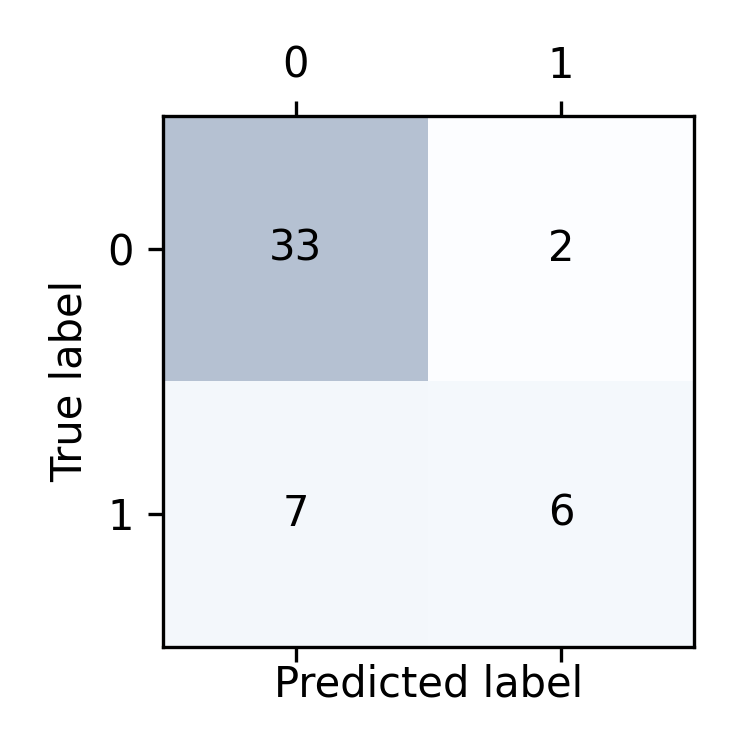
\includegraphics[keepaspectratio, scale=0.5]{fig/chapter4/wind_hateruma_1/hateruma_route_hateruma_dep_1.png}
   %2020-09-05 09/00/00_FN_setu.png
  \end{center}
  \caption{波照間航路1日前モデルの混同行列}
  \label{wind_hateruma_1_conf}
 \end{minipage}
 \begin{minipage}{0.5\hsize}
  \begin{center}
  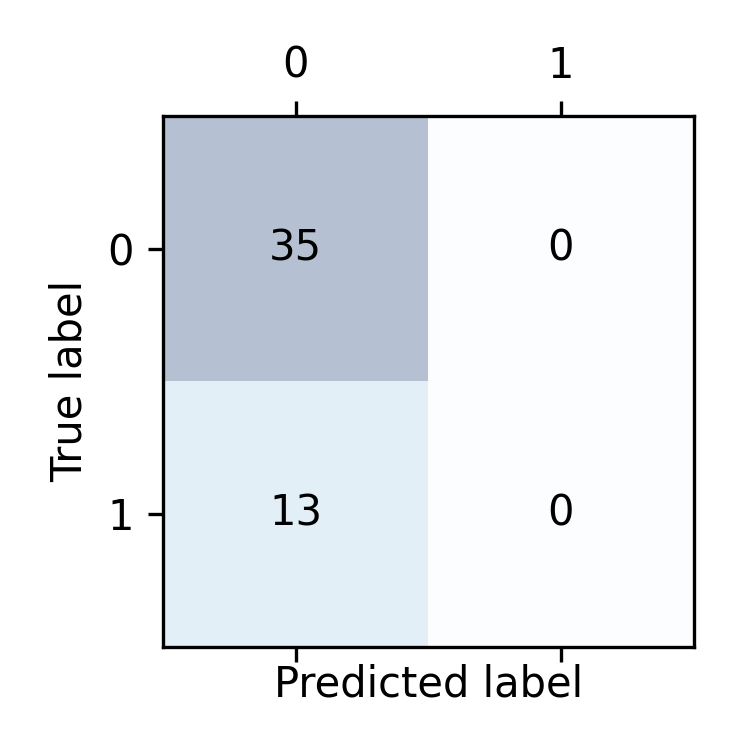
\includegraphics[keepaspectratio, scale=0.5]{fig/chapter4/wind_hateruma_2/hateruma_route_hateruma_dep_2.png}
   %2021-01-21 09/00/00_unkou_FP_setu.png
  \end{center}
   \caption{波照間航路2日前モデルの混同行列}
 \label{wind_hateruma_2_conf}
 \end{minipage}
\end{figure}

表\ref{img_wind_iriue}の西表上原航路は表\ref{img_wave_hatoma}と同様の傾向が見られた。またこれらの同様な傾向の見られた航路では8日前からF値の評価が7日前と比較して上昇していることが確認できる。8日間というスパンが教師データと画像をうまく一致するような傾向が本研究で対象とした航路に存在すると考えられる。

表\ref{img_wind_taketomi}の竹富航路でも波高レイヤーと同様に欠航データが極端に少ないため精度が良くならないことが確認できる。

\section{考察まとめ}
数値データでは、散布図により特徴量と予測ラベルの分布を示すことで、モデルの重要視している特徴量を発見できた。予測精度の悪いモデルをでは、特徴量の分布に運航時と欠航時の差異がみられない。これらは教師ラベルと特徴量の取得時間のラグがあることに起因すると考えられる。波高、風速画像ではモデルの出力した予測と入力した画像、トレーニングした画像を比較することで、その航路のモデルにおける画像と教師ラベルの関係性、特徴を解析することができた。性能が極端に低いモデルではトレーニングに使用した画像において、教師ラベルと画像の特徴に規則性がほぼ無いために、画像の特徴を捉えられなかったと考えられる。風速、波高の画像どちらもモデルに対しての影響が似ていた。これは船舶の欠航が波高の高さ、風速の大きさによって決定するためであると考えられる。また、画像モデルにおいて欠航データが十分にある航路、表\ref{img_wave_hatoma}と表\ref{img_wind_iriue}では、8日前モデルからは評価指標が上昇した。これは本研究で扱った八重山諸島の周辺の気象画像と教師データの関係性において周期性があると考察できる。
\\ これらの考察より欠航予測のための数値データ、画像データの特徴抽出は時系列を考慮したデータが望ましく、つまり予測に周期性を加味できればより高い精度の予測ができるだろう。
%その航路において周期性の情報も加味されたデータセット作成が必要である。考察できる、つまり



